\documentclass[10pt,twocolumn,letterpaper]{article}
\usepackage[accsupp]{axessibility}
%%%%%%%%% PAPER TYPE  - PLEASE UPDATE FOR FINAL VERSION
\usepackage{cvpr}      % To produce the REVIEW version
%\usepackage{cvpr}              % To produce the CAMERA-READY version
%\usepackage[pagenumbers]{cvpr} % To force page numbers, e.g. for an arXiv version

%%%%%%%%% PAPER ID  - PLEASE UPDATE
\def\cvprPaperID{11304} % *** Enter the CVPR Paper ID here
\def\confName{CVPR}
\def\confYear{2023}


\usepackage[utf8]{inputenc} % allow utf-8 input
\usepackage[T1]{fontenc}    % use 8-bit T1 fonts
\usepackage{hyperref}       % hyperlinks
\usepackage{url}            % simple URL typesetting
\usepackage{booktabs}       % professional-quality tables
\usepackage{amsfonts}       % blackboard math symbols
\usepackage{nicefrac}       % compact symbols for 1/2, etc.
\usepackage{microtype}      % microtypography
\usepackage{xcolor}         % colors

%%MY PACKAGES
\usepackage{pgfplots}
\usepackage{comment}
\usepackage{amsmath}
\usepackage{hyperref}
%\usepackage[caption=false,font=footnotesize]{subfig}
\usepackage{gensymb}
\usepackage{booktabs}
\usepackage{multirow}
\usepackage{wrapfig}
\usepackage{tabu}
\usepackage{soul}
\usepackage{floatrow}
\newfloatcommand{capbtabbox}{table}[][\FBwidth]

\newdimen\figrasterwd
\figrasterwd\columnwidth
\newcommand{\revised}[1]{{\color{black}#1}}
\newcommand{\ns}[1]{{\color{blue}#1}}
\newcommand{\mlv}[1]{{\color{purple}#1}}

\title{Data-efficient Large Scale Place Recognition with Graded Similarity Supervision}


% The \author macro works with any number of authors. There are two commands
% used to separate the names and addresses of multiple authors: \And and \AND.
%
% Using \And between authors leaves it to LaTeX to determine where to break the
% lines. Using \AND forces a line break at that point. So, if LaTeX puts 3 of 4
% authors names on the first line, and the last on the second line, try using
% \AND instead of \And before the third author name.

\author{  Mar\'ia Leyva-Vallina\\
  University of Groningen\\
{\tt\small m.leyva.vallina@rug.nl}
\and
 Nicola Strisciuglio \\
University of Twente \\
{\tt\small n.strisciuglio@utwente.nl}
\and
   Nicolai Petkov \\
   University of Groningen \\
{\tt\small n.petkov@rug.nl}
}


% \pgfplotsset{compat=1.18}
\begin{document}


\maketitle


\begin{abstract}
Visual place recognition (VPR) is a fundamental task of computer vision for visual localization. Existing methods are trained using image pairs that either depict the same place or not. Such a binary indication does not consider continuous relations of similarity between images of the same place taken from different positions, determined by the continuous nature of camera pose. The binary similarity induces a noisy supervision signal into the training of VPR methods, which stall in local minima and require expensive hard mining algorithms to guarantee convergence. Motivated by the fact that two images of the same place only partially share visual cues due to camera pose differences, we deploy an automatic re-annotation strategy to re-label VPR datasets. We compute graded similarity labels for image pairs based on available localization metadata. Furthermore, we propose a new Generalized Contrastive Loss (GCL) that uses graded similarity labels for training contrastive networks. We demonstrate that the use of the new labels and GCL allow to dispense from hard-pair mining, and to train image descriptors that perform better in VPR by nearest neighbor search, obtaining superior or comparable results than methods that require expensive hard-pair mining and re-ranking techniques. 


%This affects the training of VPR methods, that usually stall in local minima and are thus coupled with expensive pair-mining strategies to select hard training pairs properly. Motivated by this, we propose automatic methods to re-label VPR datasets and exploit camera pose metadata or 3D information as proxy to estimate a graded similarity of image pair. 
%achieves

%We demonstrate that graded similarity labels can be used to compose training batches instead of using hard-pair mining, with a speed-up of the training up to $\sim$200x faster that existing methods. 

%\st{Visual place recognition is a challenging task of computer vision and a key component of visual-based localization and navigation systems.  State-of-the-art models are trained using image pairs or triplets labeled as \emph{similar} or \emph{dissimilar}, in a binary fashion. In practice, however, the similarity between two images is continuous rather than binary. Furthermore, training these models is computationally complex and involves costly hard-negative pair and triplet mining.  We propose a Generalized Contrastive loss (GCL) function for metric learning that exploits continuous image similarity to train siamese networks. We use camera position and orientation to re-annotate the MSLS dataset with the degree of similarity of image pairs. Siamese networks trained with the GCL function consistently outperform their counterparts trained using the traditional  contrastive loss. They achieve superior performance than more complex state-of-the-art approaches that use triplet loss, pair mining and re-ranking, and generalize well to unseen datasets. We do not use pair mining, considerably reducing memory and computation requirements compared to existing methods (5 hours to train a VGG backbone with GLC compared to 45 days to train a VGG-NetVLAD model, on an NVidia V100 gpu). The source code and MSLS re-annotation will be released.}
\end{abstract}



\section{Introduction}
\section{Introduction}
\label{sec:intro}
\begin{figure}[t]
\begin{center}
    \includegraphics[width=1\linewidth]{figures/teaser.pdf}
\end{center}
\vspace{-0.1in}
\caption{\textbf{{\em Foggy} vs {\em Clear} NeRF.} Our \ournerf gets rid of reconstruction errors manifested as foggy ``floaters" in the density volume without additional input or significant computational overhead. 
%
Below are density profiles along a given ray before and after our geometry correction procedure, where we discard density peaks corresponding to floaters.
}
\label{fig:teaser}
\vspace{-0.2in}
\end{figure}



%The emergence of 
Neural Radiance Fields (NeRFs)~\cite{mildenhall2020nerf}  %and its variants 
have made revolutionary contributions in %photo-realistic 
novel view synthesis~\cite{barron2021mip,barron2022mip}, 
autonomous driving~\cite{rematas2022urban,tancik2022block}, digital human~\cite{hong2022headnerf,zhao2022humannerf}, and 3D content generation~\cite{eg3d,poole2022dreamfusion,lin2022magic3d}.
%by leveraging a multi-layer perceptron (MLP) to implicitly model the mapping from input 5D coordinates (i.e., 3D coordinates $\mathbf{x} = (x,y,z)$ and 2D viewing directions $\mathbf{d}=(\theta,\phi)$) to volume density $\sigma$ and view-dependent emitted radiance color $\mathbf{c} = (r,g,b)$. 
%
%They then use traditional volume rendering mechanisms on the obtained continuous 5D function (i.e., MLP) to generate novel views. 
To date, unfortunately, most NeRF-based methods encounter challenges when tackling large-scale cluttered scenes (e.g., Fig.~\ref{fig:teaser}):
\begin{enumerate}[leftmargin=0.16in, topsep=2pt,itemsep=-1ex,partopsep=1ex,parsep=1ex]
\item Input observations used for NeRF are often too sparse  compared to forward-facing or synthetic looking-inward scenes;
%\item Recovering fine-grained objects within a large volume is challenging for NeRF; %in capturing details accurately.
\item View-dependent visual effects give rise to ambiguity, resulting in a ``foggy" density field as shown in Fig.~\ref{fig:teaser}. 
%
Such artifacts are particularly pronounced in indoor scenes strewn with view-dependent appearances, such as specular highlights, glossy surface reflections from man-made objects. 
\end{enumerate}

Despite attempts to enhance NeRF's rendering quality given suboptimal input, such as using 3D conical frustums~\cite{barron2021mip,barron2022mip}, physically-grounded augmentations~\cite{chen2022aug}, and misalignment correction~\cite{jiang2022alignerf},  these challenges have yet to be fully resolved.
%
Depth supervision~\cite{deng2022depth, wei2021nerfingmvs} or proxy geometry~\cite{xu2021scalable,wu2022scalable} images can help alleviate the challenges in handling large-scale with sparse input, at the expense of %but they come at the cost of requiring 
expensive pre-processing or additional input.
%
Another line of work~\cite{wang2021neus, oechsle2021unisurf, wang2022neuris} achieves better reconstruction of surface geometry by using signed distances instead of volume density as scene representation. However, they sacrifice the ability to synthesize photo-realistic novel views.

%We observe that NeRF has been suffering from foggy ``floater" artifacts in large-scale cluttered scenes.
%
%Such artifacts are particularly pronounced in indoor scenes strewn with view-dependent appearances from man-made objects. 
%
To address the above issues, we propose an extension to NeRF, dubbed as {\bf \ournerf}, which enforces effective {\em appearance} and {\em geometry} constraints conducive to accurate colors and 3D densities estimation. We believe \ournerf can contribute beyond novel view synthesis, such as NeRF object detection~\cite{hu2022nerf}, NeRF object segmentation~\cite{zhi2021place, liu2022unsupervised, fan2022nerf,ren2022neural}, and NeRF registration~\cite{goli2022nerf2nerf}, where the rooms for improvement are substantial if more accurate color and density estimation are available.

Correspondingly, there are two steps in \ournerf. First, for appearance correction, the view-independent and view-dependent color components are predicted from the underlying 3D scene, which is combined to produce the final color estimation (Fig.~\ref{fig:toaster}).
%
The view-independent component (diffuse color and shading) captures the overall scene color, while the view-dependent component (highlights or reflections) captures color variations due to changes in viewing angle.
%
\ournerf then discards these view-dependent appearances in the training views to prevent them from interfering with the density estimation.
%
Second, a simple and effective geometry correction procedure will be performed to further eliminate the foggy ``floaters" or density errors. This geometry correction procedure is based on an assumption in line with traditional ray tracing in computer graphics.
\begin{comment}
% xh: basically copying method
On the other hand, ClearNeRF performs a geometric correction procedure performed on each traced ray during inference to refine the density estimation and better tackle the floater artifacts. 
%
The geometry correction procedure assumes that there should only be one salient peak along each traced ray during NeRF inference. 
Only the salient peak closest to the ray origin (the camera center) corresponds to  true geometry while the others will be manifested as foggy floaters hovering in the density volume. 
%
This assumption is in line with traditional ray tracing in computer graphics where in the absence of noise, only one intersection per ray should be returned to indicate the closest ray-object intersection.
%
\end{comment}
%%%%%%%%%%%
%As shown in Fig.~\ref{fig:teaser}, when reconstructing an indoor scene with sparse input and highly view-dependent objects, NeRF produces severe floating artifacts due to its attempt to explain view-dependent appearances.
%
Experiments verify that our proposed \ournerf can effectively get rid of floater artifacts without additional input.% or significant computational overhead. 


In summary, our contributions include the following:
\begin{itemize}[leftmargin=0.16in, topsep=2pt,itemsep=-1ex,partopsep=1ex,parsep=1ex]
    \item We propose a concise method for decomposing view-independent and view-dependent appearance during NeRF training and eliminate the interference of view-dependent appearance.
    \item We propose a geometric correction procedure performed on each traced ray during inference to refine the density estimation and better tackle the floater artifacts.
    \item Extensive experiments and ablations verify the effectiveness of our core designs and results in improvements over the vanilla NeRF and other state-of-the-art alternatives.
    %without additional computational resources or other inputs.
\end{itemize}




%\section{Related works}

\section{Related works}
 
\noindent\textbf{Place recognition as image retrieval.} 
Visual place recognition is widely addressed as a metric learning problem, in which the descriptors of images of a place are learned to be close together in a latent space~\cite{milford15metric}. Existing methods optimize ranking loss functions, such as contrastive, triplet or average precision~\cite{radenovic2018fine,Gordo2017,revaud2019learning}. An extensive  benchmark of different approaches is in~\cite{Berton2022Bench}.
NetVLAD~\cite{Arandjelovic2017} is milestone of VPR and builds on a triplet network with an end-to-end trainable VLAD layer. It requires a computationally- and memory-expensive hard-pair mining to compose proper batches and guarantee convergence. 
SARE~\cite{liu2019stochastic} uses a NetVLAD backbone trained with a probabilistic attractive and repulsive mechanism, also making use of hard-pair mining. %While hard-pair mining addresses issues of the training stalling in local minima due to noisy binary labels~\cite{Arandjelovic2017}, we argue that batch composition can be effectively addressed before training. For instance, we use image metadata, such as GPS and compass angle, to estimate the graded similarity of image pairs, and subsequently use it to balance the distribution of hard- and easy-pairs in the training batches. 
Hard-pair mining addresses issues of the training stalling in local minima due to noisy binary labels, and is used to compose the training batches so that hard pairs are selected for the training~\cite{Arandjelovic2017}. We instead use image metadata (e.g. camera pose as GPS and compass) to a-priori estimate the graded similarity of image pairs, and subsequently use it to balance hard- and easy-pairs in the training batches. This allows to train VPR models using the graded similarity of images and avoiding hard-pair mining.

Training with noisy binary labels produces image descriptors with drawbacks in nearest neighbor search retrieval, and re-ranking algorithms are necessary to post-process the retrieved results and increase VPR performance~\cite{delg,sarlin20superglue}. Patch-NetVLAD~\cite{hausler2021patch} builds on a NetVLAD backbone and performs multi-scale aggregation of NetVLAD descriptors to re-rank retrieval results. A transformer architecture named TransVPR was trained using a triplet loss function and hard-pair mining in~\cite{wang2022transvpr}. The retrieval step is combined with a costly re-ranking strategy to improve the retrieval results. We instead focus on using  more informative and robust image pair labels to avoid noisy training and obtain more effective image descriptors for nearest neighbor search, with no necessity of performing re-ranking.

%re-ranking is used to overcome weaknesses of the learned representations in nearest neighbor search at the cost of extra processing~\cite{hausler2021patch,wang2022transvpr}.


 
\noindent\textbf{Image graded similarity. } 
Soft assignment to positive and negative classes of image pairs was investigated in~\cite{thoma2020soft}, where weighting of the assignment was based on the Euclidean distance between the GPS coordinates associated to the images. As the GPS distance induced label noise in the training process, hard-negative pair mining was still necessary to train VPR networks.
In~\cite{SFRS}, image region similarity was coupled with the GPS weak labels in a self-supervised framework to mine hard positive samples. In~\cite{berton22cosplace}, the authors formulated the VPR metric learning as a classification problem, splitting image training into classes based on similar GPS locations  to facilitate large-scale city-wide recognition.
Camera pose was used in~\cite{balntas2018relocnet} to estimate the camera frustum overlap and regress descriptors for camera (re-)localization in small-scale (indoor) environments. 
%Some attempts to include partial similarity information were done to train descriptors for relative pose estimation and camera localization in RelocNet and CamNet~\cite{ding2019camnet}, where the camera frustum overlap is used as a target to regress the relative pose of cameras. 
In~\cite{kim2021embedding}, a weighting scheme for the contrastive loss function is proposed as a function of the distance in the latent space, which requires an extra step of normalization of the distances to avoid a divergent training. In this work, we relabel VPR datasets using camera pose and field of view overlap, or ratio of shared 3D surface as proxies to estimate the graded similarity of training image pairs. We compute the new labels once, and use them to select the training batches and directly in the optimization of the networks to obtain effective descriptors for VPR in a data-efficient manner.


\noindent\textbf{Relation and difference with prior works. } We undertake a different direction than previous works, and propose a simplified way to learn image descriptors for retrieval-based VPR. We use contrastive architectures without hard-pair mining and exploit the graded similarity of image pairs to learn robust descriptors.
Instead of developing algorithmic solutions (e.g. hard-pair mining or re-ranking) to achieve better VPR results by increasing the complexity of the methods,  %, to , that is better retrieved results in a nearest-neighbor retrieval scheme. 
we focus on data-efficiency and improve similarity labels to better exploit the training data. This allows to purposely keep the complexity of the architecture simpler (a convolutional backbone and a straightforward pooling strategy) than other methods. We apply prior knowledge and use metadata about the position and orientation of the cameras to estimate a more robust ground truth image similarity that enables to drop expensive hard-mining procedures and train (bigger) networks efficiently. We show that this approach leads to reduced training time and very robust descriptors that perform well in nearest neighbour search with no need of re-ranking.


%In this light, we showed that for place recognition we can achieve very high results (in some cases better than sota), without the need of complicating the models, but with a wiser use of the data and labels.



%\section{Methodology}
\chapter{Methodology}\label{section:method}

This section explains the theoretical details of the models used in the experiments. These are the regular vanilla variational autoencoder (VAE), the Riemannian Hamiltonian variational autoencoder (RH-VAE), the spherical variational autoencoder (\svae) and the roto-equivariant Variational Auto-Encoder (KS-VAE).

\section{Variational Autoencoder} \label{subsec:vae}
At the basis of all models used in this work lies the autoencoder model. 
The general framework of an autoencoder consists of two neural networks: an encoder that encodes an input image $x$ into a lower-dimensional latent representation $z$, and a decoder that decodes the latent representation into a reconstruction $\hat{x}$, with the aim of minimizing the error between the original image and its reconstruction. The Variational Autoencoder (VAE) \citep{maxkingma2013auto} is a generative version of the original autoencoder, that instead of learning the latent representation $z$ directly, learns a distribution describing each data point, from which the latent representation is sampled (see Figure \ref{autoencoders}). The aim of the VAE is therefore to learn a parameterized probability distribution $p_{\theta }$ describing the input data $x$'s true distribution $P(x)$. To do so, we assume that the input data can be characterized by a lower-dimensional latent distribution $z$. The marginal likelihood can then be written as \begin{align} p_\theta(x) = \int p_\theta(x|z)q_{prior}(z)dz\end{align} where $q_{prior}(z)dz$ is a prior distribution over the latent variables, that in case of the vanilla VAE is chosen as a standard normal Gaussian distribution. 
Unfortunately, computing $p_\theta(x)$ involves the posterior $p_\theta(z|x)$, which is computationally expensive and often intractable.
We therefore introduce an approximation $q_\phi(z|x)$ of the true posterior, which is computed by a neural network: the encoder. We can then train a variational autoencoder, consisting of the encoder, which computes the approximate posterior and the decoder, which computes the conditional likelihood $p_\theta(x|z)$.

Within the variational autoencoder framework, the encoder and decoder are optimized in a joint setting. To find the posterior distribution $q_\phi(z|x)$ that best approximates the true posterior $p_\theta(z|x)$, we can use the \textit{Kullback-Leibler} divergence, which measures the difference between two probability distributions. Ideally, we would want to minimize this term, which is given by

\begin{align}
    \text{KL}(q_{\boldsymbol{\mathbf{\phi}}}(\boldsymbol{\mathbf{z}}\mid \boldsymbol{\mathbf{x}})\,\,||\,\,p_{\boldsymbol{\mathbf{\theta}}}(\boldsymbol{\mathbf{z}}\mid \boldsymbol{\mathbf{x}}))
    &= \mathbb{E}_{q_\phi} \big[ \log q_\phi(\mathbf{z}) \big] - \mathbb{E}_{q_\phi} \big[ \log p_\theta(\mathbf{z} | \mathbf{x}) \big]\\
    &= \mathbb{E}_{q_\phi} \big[ \log q_\phi(\mathbf{z}) \big] - \mathbb{E}_{q_\phi} \bigg[ \log \frac{p_\theta(\mathbf{x}, \mathbf{z}) }{p_\theta(\mathbf{x})} \bigg]\\
    &= \mathbb{E}_{q_\phi} \big[ \log q_\phi(\mathbf{z}) \big] - \mathbb{E}_{q_\phi} \big[ \log p_\theta(\mathbf{x}, \mathbf{z}) - \log p_\theta(\mathbf{x}) \big]\\
    &= \mathbb{E}_{q_\phi} \big[ \log q_\phi(\mathbf{z}) - \log p_\theta(\mathbf{x}, \mathbf{z}) \big] + \mathbb{E}_{q_\phi} \big[ \log p_\theta(\mathbf{x}) \big]\\
    &= \mathbb{E}_{q_\phi} \big[ \log q_\phi(\mathbf{z}) - \log p_\theta(\mathbf{x}, \mathbf{z}) \big] + \underbrace{\log p_\theta(\mathbf{x})}_{\text{intractable}}.
\end{align}

% \begin{figure}[h]
%     \centering
%     \subfloat[\centering Autoencoder]{{\includegraphics[width=0.43\textwidth]{images/method/ae.png} }}%
%     \qquad
%     \subfloat[\centering Variational Autoencoder]{{\includegraphics[width=0.5\textwidth]{images/method/vae} }}%
%     \caption{Schematic view of autoencoder and variational autoencoder architectures. The encoder either learns to map the input vector $\mathbf{x}$ to a latent vector $\mathbf{z}$ directly (AE), or learns the parameters of a distribution describing $\mathbf{x}$, from which $\mathbf{z}$ is then sampled (VAE). The decoder in both cases learns to most accurately reconstruct the original input ($\mathbf{\hat{x}}$) from $\mathbf{z}$.}
%     \label{autoencoders}
% \end{figure}
\begin{figure}[h]
    \centering
    \subfloat[\centering Autoencoder]{{\includegraphics[width=0.36\textwidth]{images/method/ae_colored.png} }}%
    \quad \quad \quad
    \subfloat[\centering Variational Autoencoder]{{\includegraphics[width=0.5\textwidth]{images/method/vae_colored1.png} }}%
    \caption{Schematic view of autoencoder and variational autoencoder architectures. The encoder either learns to map the input vector $\mathbf{x}$ to a latent vector $\mathbf{z}$ directly (AE), or learns the parameters of a distribution describing $\mathbf{x}$, from which $\mathbf{z}$ is then sampled (VAE). The decoder in both cases learns to most accurately reconstruct the original input ($\mathbf{\hat{x}}$) from $\mathbf{z}$.}
    \label{autoencoders}
\end{figure}

However, as can be seen when we rewrite the equation, we still have the intractable evidence term $\log p_\theta(\mathbf{x})$. We therefore introduce a lower bound of the log-likelihood using Jensen’s inequality. 
\begin{align}
    \log p_\theta (x) &=\log \int_{\mathbf{z}} p_\theta(\mathbf{x}, \mathbf{z}) \\
    &=\log \int_{\mathbf{z}} p_\theta(\mathbf{x}, \mathbf{z}) \frac{q_\phi(\mathbf{z})}{q_\phi(\mathbf{z})} \\
    &=\log \left(\mathbb{E}_{q_\phi}\left[\frac{p_\theta(\mathbf{x}, \mathbf{z})}{q_\phi(\mathbf{z})}\right]\right) \\
    & \geq \underbrace{\mathbb{E}_{q_\phi}[\log p_\theta(\mathbf{x}, \mathbf{z})]-\mathbb{E}_{q_\phi}[\log q_\phi(\mathbf{z})]}_\text{ELBO} 
\end{align}
This lower bound is called the Evidence Lower BOund (ELBO) \citep{maxkingma2013auto}. Because the evidence is a constant, maximizing the ELBO amounts to minimizing the KL divergence. The ELBO therefore forms the key to variational inference: instead of finding our optimal distribution q by minimizing the KL divergence, requiring us to calculate the intractable evidence term, we find it by maximizing ELBO, which is a tractable operation. We can therefore use the ELBO as our model's loss function. 
To arrive at our final loss function, we rearrange the ELBO term into the following expression

\begin{align}
    \text{ELBO} &= \mathbb{E}_{q_\phi}[\log p_\theta(\mathbf{x}, \mathbf{z})]-\mathbb{E}_{q_\phi}[\log q_\phi(\mathbf{z})] \\
    &= \mathbb{E}_{q_\phi}[\log p_\theta(\mathbf{x}, \mathbf{z}) - \log q_\phi(\mathbf{z})] \\
    &= \mathbb{E}_{q_\phi}[\log p_\theta(\mathbf{x}| \mathbf{z}) + \log p_\theta(\mathbf{z})
    - \log q_\phi(\mathbf{z})] \\
    &= -\mathbb{E}_{q_\phi}[\log p_\theta(\mathbf{x}| \mathbf{z}) - \mathbb{E}_{q_\phi}[\log p_\theta(\mathbf{z}) - \log q_\phi(\mathbf{z})] \\
    &= -\mathbb{E}_{q_\phi}[\log p_\theta(\mathbf{x}| \mathbf{z})] - \text{KL} \left(q_{\boldsymbol{\mathbf{\phi}}}\left(\boldsymbol{\mathbf{z}}\mid \boldsymbol{\mathbf{x}})\,\,||\,\,p_{\boldsymbol{\mathbf{\theta}}}(\boldsymbol{\mathbf{z}}\right)\right),
\end{align}

which consists of a regularization term $\mathbb{E}_{q_\phi}[\log p_\theta(\mathbf{x}| \mathbf{z})]$ and a KL divergence 
term $\text{KL} \left(q_{\boldsymbol{\mathbf{\phi}}}\left(\boldsymbol{\mathbf{z}}\mid \boldsymbol{\mathbf{x}})\,\,||\,\,p_{\boldsymbol{\mathbf{\theta}}}(\boldsymbol{\mathbf{z}}\right)\right)$. The expectation term is also called the \textit{reconstruction loss}. It pushes the model to most accurately reconstruct an image from its encoded latent representation, such that the difference between decoding a sampled latent vector from the learned distribution is as small as possible. Meanwhile, the KL divergence term is also called the \textit{regularization loss}, as it pushes the approximate posterior to more closely resemble the prior distribution. When choosing a normal Gaussian distribution for both the prior and approximate posterior, as is the standard for VAEs, the prior enforces the posterior probability mass to have spread like a Gaussian, therefore adding a form of regularization to the model. Moreover, for a Gaussian prior and posterior, the KL term reduces to a closed-form formula, making computations more efficient. 



Now, all that remains is to solve the problem of the random sampling operation from $\mathbf{z}$ not being differentiable. \citeauthor{maxkingma2013auto} propose to solve this by using the \textit{reparameterization trick}, which suggests that instead of sampling $\mathbf{z}$ directly, some noise $\epsilon$ is sampled from a unit Gaussian distribution. We can then add the learned mean parameter $\mu$ to this noise term and multiply it by the variance $\sigma$ to arrive at a mean and variance as would have been directly sampled from the latent distribution, while still allowing for backpropagation through the neural network. 



% https://mpatacchiola.github.io/blog/2021/01/25/intro-variational-inference.html
% --------------------------------------------
% --------RIEMANNIAN RHVAE--------------------
% --------------------------------------------

\section{Riemannian Variational Autoencoder}\label{subsec:rhvae}
As discussed in Section \ref{bg:dst}, the vanilla variational autoencoder suffers from a distortion in the latent space  as a consequence of the Euclidean manifold assumption and Gaussian prior, which makes geometric notions such as distance unreliable in this space. One way of remedying this problem is to use metrics defined in the non-distorted input space instead, and mapping them to the manifold space. Such a mapping is possible by endowing the manifold with a Riemannian metric. A model that not only does this, but also \textit{learns} a fitting metric from the input data, is the Riemannian Hamiltonian VAE. These qualities make it a promising technique for accurately representing relationships between points and modelling BE progression.

The following section describes the details of RHVAE. Before this can be discussed however, it is important to give the reader a short overview of the basics of Riemannian geometry.

    \subsection{Basics of Riemannian Geometry}
        As discussed earlier, a real, smooth manifold is a space that is locally similar to a linear space. Riemannian geometry allows for defining notions of angles, distances, and volume on such spaces by endowing the manifold with a \textit{Riemannian Metric}. The manifold can then be considered as a \textit{Riemannian manifold}.
        We define an $m$-dimensional Riemannian manifold embedded in an ambient Euclidean space $\mathcal{X} = \mathbf{R}^d$ and endowed with a \textit{Riemannian metric} $\mathbf{G} \triangleq (\mathbf{G}_{\mathbf{x}})_{\mathbf{x} \in \mathcal{M}}$ to be a smooth curved space $(\mathcal{M},G)$. 
        For every point on the manifold $\mathcal{M}$, there exists a tangent vector $\mathbf{v}\in \mathcal{X}$ that is tangent to $\mathcal{M}$ at $\mathbf{x}$ iff there exists a smooth curve $\gamma:[0,1] \mapsto \mathcal{M}$ such that $\gamma(0)=\mathbf{x}$ and $\dot{\gamma}(0)=\mathbf{v}$.
        The velocities of all such curves through $\mathbf{x}$ form the \emph{tangent space} $\mathcal{T}_{\mathbf{x}}\mathcal{M}=\{ \dot{\gamma} (0) \,|\, \gamma:\mathbf{R}\mapsto\mathcal{M} \text{ is smooth around $0$ and } \gamma(0)=\mathbf{x}\}$, which has the same dimensionality as the manifold. The tangent space can be viewed as the collection of all the different ways in which the points on the manifold can be passed. 
        
        \begin{figure}[H]
            \centering
            \includegraphics[width=0.4\textwidth]{images/method/Manifold_Example.png}
            \caption{Schematic example of a 2-D manifold $\mathcal{M}$ and its tangent space $\mathcal{M}_x \mathcal{T}$ at point $x$. The geodesic $\gamma(t)$ starts at $x$ and goes in the direction $\mathbf{v}$.}
            \label{fig:my_label}
        \end{figure}
        
        The Riemannian metric $G(\cdot)$ then equips each point $\mathbf{x}$ on the manifold with an inner product in the tangent space $\mathcal{T}_{\mathbf{x}}\mathcal{M}$, \textit{e}.\textit{g}. $\langle \mathbf{u}, \mathbf{v} \rangle_x = \mathbf{u} ^T \mathbf{G}_{\mathbf{x}} \mathbf{v}$. 
        This induces a norm $\|\mathbf{u}\|_\mathbf{x}\,,\forall \mathbf{u} \in \mathcal{T}_{\mathbf{x}}\mathcal{M}$ locally defining the geometry of the manifold. Given these local notions, we can not only compute local angles, lengths, and areas, but also derive global quantities by integrating over local properties. We can thus compute the length of any curve on the manifold $\gamma : [0,1] \rightarrow \mathcal{M}$, with $\gamma(0) = \mathbf{x}$ and $\gamma(1) = \mathbf{y}$ as the integral of its speed: $\ell(\gamma) = \int_{0}^1 \|\dot{\gamma}(t)\|_{\gamma(t)}dt$.
        The notion of length leads to a natural notion of distance by taking the infimum over all lengths of such curves, giving the \emph{gobal Riemannian distance} on $\mathcal{M}$, $d(\mathbf{x},\mathbf{y})=\inf_{\gamma}\ell(\gamma)$. The constant speed-length that minimizes the distance of a curve between two points is called a \emph{geodesic} on $\mathcal{M}$. VAEs can generate images along such a geodesic path, providing a more geometry-aware alternative to the vanilla VAE's linear interpolations.

           
    \subsection{Riemannian Hamiltonian Variational Autoencoder}
    \citeauthor{chadebec2020geometryaware} propose the Riemannian Hamiltonian VAE (RHVAE), which assumes the latent space to be structured as a Riemannian manifold $\mathcal{M}=\left(\mathbb{R}^{d}, \mathbf{G}\right)$ with $\mathbf{G}$ being the Riemannian metric, as described above. RHVAE attempts to exploit this assumed Riemannian structuring by introducing two main extensions of the vanilla VAE. First, to replace the regular Gaussian posterior distribution with a geometrically-informed posterior through the use of Riemannian Hamiltonian dynamics. Secondly, to find an appropriate Riemannian metric for this space, by learning it with a neural network. 
    
    \subsubsection{Learning the Riemannian Metric}
    As mentioned in section \ref{bg:rie}, while the choice of Riemannian metric is crucial to defining the manifold space, the computation of many proposed metrics involves the Jacobian, which is difficult and expensive to compute. In the RHVAE framework, the metric is therefore proposed to be learned directly from the data. This parameterized metric is defined as follows

    \begin{align}\label{eq:riemanmetric}
            \mathbf{G}^{-1}(z)=\sum_{i=1}^{N} L_{\psi_{i}} L_{\psi_{i}}^{\top} \exp \left(-\frac{\left\|z-c_{i}\right\|_{2}^{2}}{T^{2}}\right)+\lambda I_{d},    
    \end{align}

    
    
    where $N$ is the number of observed data points, $L_{\psi_{i}}$ are parameterized lower triangular matrices with positive diagonal coefficients learned from the data through neural networks, $c_{i}$ are centroids corresponding to the mean of the encoded distributions for every data point, 
    $T$ is a temperature parameter that scales the metric close to the centroids and $\lambda$ is a regularization factor, which allows for scaling the Riemannian volume element further away from the data. The above-defined metric is smooth, differentiable, and allows for computing geodesics easily, which is useful for creating informed interpolations along the geodesic curve on the manifold. 
    % The shape of this metric is very powerful since we have access to a closed-form expression of the inverse metric tensor which is usually useful to compute shortest paths (through the exponential map). Moreover, this metric is very smooth, differentiable everywhere and allows scaling the Riemannian volume element $\sqrt{\operatorname{det} \mathbf{G}(z)}$ far from the data very easily through the regularization factor $\lambda$.

    Training of the metric learning model is done jointly with training the rest of the RHVAE network. Just as with a regular VAE, an input image is encoded by the encoder network, which learns the parameters of a normal Gaussian distribution $\mathcal{N}(\mu, \sigma^2)$. Simultaneously, the metric network learns to map the input image to the lower triangular matrix $L_{\psi_{i}}$, allowing us to compute the Riemannian metric. These serve as input for a sampler, called the RHMC (Riemmanian Hamiltonian Monte-Carlo) sampler, from which a latent vector $z$ defined on the manifold  $z \in \mathcal{M}$ is sampled. The RHMC sampler thus essentially enriches the Gaussian approximate posterior function to be more aware of the underlying geometry of the manifold. 

    \subsubsection{A Geometrically-Aware Posterior through the RHMC Sampler}
    % For RHVAE, we assume that the latent space is the Riemannian manifold $\mathcal{M}=\left(\mathbb{R}^{d}, \mathbf{G}\right)$ with $\mathbf{G}$ being the Riemannian metric. 
    
    % Building upon the Hamiltonian VAE (HVAE) [52], we propose to exploit the assumed Riemannian structure of the latent space by using Riemannian Hamiltonian dynamics [74] instead. The main goal remains the same and consists in using the Riemannian Hamiltonian Monte Carlo (RHMC) sampler to be able to enrich the variational posterior $q_{\phi}(z \mid x)$ such that it targets the true (unknown) posterior $p_{\theta}(z \mid x)$ while exploiting the properties of Riemannian manifolds.
    Given the Riemannian manifold $\mathcal{M}=\left(\mathbb{R}^{d}, \mathbf{G}\right)$ with our metric $\mathbf{G}$, we want to sample our latent $z$ from a distribution that is informed about the geometry of the Riemannian latent space. We therefore want to obtain this target distribution $p_{\text {target }}(z)$ through the Riemannian Hamiltonian dynamics of the RHMC sampler. 
    The core of this sampling process revolves around the concept of seeing the VAE as an energy-based model, where $z$ is seen as the position of a traveling particle in $\mathcal{M}$. We also sample a random variable $v$, which represents the velocity of this particle. Following the view of the $z$ as a particle on a manifold, we aim to essentially simulate the evolution of the traveling particle towards the target density $p_{\text {target }}(z)$ using a Markov Chain.
    We first define the potential energy $U(z)$ and kinetic energy $K(z, v)$ as   

    \begin{align}
    U(z) & =-\log p_{\text {target }}(z) \\
    K(v, z) & =\frac{1}{2}\left[\log \left((2 \pi)^{d}|\mathbf{G}(z)|\right)+v^{\top} \mathbf{G}^{-1}(z) v\right] ,
    \intertext{which together give the Hamiltonian}
    H(z,v) &= U(z) + K(v,z) .
    \end{align}
    
    This Hamiltonian equation is integrated in every step of the Markov chain, which allows us to preserve  the target density and make sure that the chain eventually converges to the stationary target distribution. 
    This essentially creates a flow that is informed both by the target distribution and by the latent space geometry thanks to the Riemannian metric $\mathbf{G}$. The approximate posterior distribution is guided by this flow, leading to better variational posterior estimates.


% -------------------------------------------------------------------------------------------------------
% --------------HYPERSPHERICAL---------------------------------------------------------------------------
% -------------------------------------------------------------------------------------------------------


\section{Hyperspherical Variational Autoencoder}\label{subsec:svae}
Another approach to solving the distortion of the latent space is to structure it as a hyperspherical manifold and assume a uniform prior. 
One of the discussed issues with vanilla variational autoencoders is that the Gaussian prior tends to concentrate points in a cluster around the center of the distribution's probability mass. In the case of multi-class data, this can become problematic, as separate clusters in the latent space will also be pulled towards the origin and therefore become difficult to separate. In an ideal case, we would still have a prior that regularizes the approximate posterior, but that does not enforce the encoded points to be at the center of the probability mass. The probability distribution that does exactly this is the uniform prior. Instead of concentrating points in one location, it spreads them over the latent space. However, the vanilla VAE's Gaussian posterior means that our latent space corresponds to a Euclidean hyperplane, a space on which the uniform prior is not well-defined. 

\subsubsection{Replacing the Gaussian by the von Mises-Fisher Distribution}
By assuming a \textit{hyperspherical} posterior, however, our latent manifold becomes a compact space on which it is possible to define a uniform prior. This is why \svae uses a von Mises-Fisher (vMF) distribution instead of the Gaussian posterior of the vanilla VAE. The vMF distribution is often considered analogous to the Gaussian distribution on a hypersphere of dimensionality $m$. Similarly to the Gaussian, it is parameterized by a mean direction $\mu \in \mathbb{R}^{m}$, but instead of variance, the vMF is parameterized by a concentration parameter around the mean $\kappa \in \mathbb{R}_{\geq 0}$. The parameters $\mu$ and $\kappa$ are called the mean direction and concentration parameter, respectively. The greater the value of $\kappa$, the higher the concentration of the distribution around the mean direction $\mu$. The distribution is unimodal for $\kappa > 0$ and is uniform on the sphere for $\kappa$ = 0. 
The probability density function of the vMF distribution for a random unit vector $\mathbf{z}$ is then defined as

\begin{align}
q(\mathbf{z} \mid \mu, \kappa) & =\frac{\kappa^{m / 2-1}}{(2 \pi)^{m / 2} \mathcal{I}_{m / 2-1}(\kappa)} \exp \left(\kappa \mu^{T} \mathbf{z}\right),
\end{align}

where the mean direction $\mu$ is a unit vector $(\|\mu\| = 1)$ and
% $\|\mu\|^{2}=1, \mathcal{C}_{m}(\kappa)$ is the normalizing constant, and 
$\mathcal{I}_{n}(\kappa)$ denotes the modified Bessel function of the first kind at order $n = (m/2-1)$.

For the special case of $\kappa=0$, the vMF represents a Uniform distribution on the $(m - 1)$-dimensional hypersphere $U\left(\mathcal{S}^{m-1}\right)$. This fact allows us to place the desired uniform prior over the hyperspherical latent space. To incorporate the newly chosen prior and posterior distribution, the KL divergence term to be optimized needs to be rewritten to

\begin{align}
    K L\left(\operatorname{vMF}(\mu, \kappa) \| U\left(\mathcal{S}^{m-1}\right)\right) &= \kappa \cdot \frac{\mathcal{I}_{m / 2}(k)}{\mathcal{I}_{m / 2-1}(k)}+\log \mathcal{C}_{m}(\kappa)-\log \left(\frac{2\left(\pi^{m / 2}\right)}{\Gamma(m / 2)}\right)^{-1},
\end{align}

Using the above as our regularization loss and Mean Squared Error (MSE) as reconstruction loss, we have defined a loss function of the hyperspherical VAE. 
% Notice that since the KL term does not depend on $\mu$, this is only optimized in the reconstruction term. The above expression cannot be handled by automatic differentiation packages because of the modified Bessel function in $\mathcal{C}_{m}(\kappa)$. Thus, to optimize this term we derive the gradient with respect to the 
% concentration parameter $\nabla_{\kappa} K L\left(\operatorname{vMF}(\mu, \kappa) \| U\left(S^{m-1}\right)\right)$ :
% $$
% \begin{align}
% & \frac{1}{2} k\left(\frac{\mathcal{I}_{m / 2+1}(k)}{\mathcal{I}_{m / 2-1}(k)}+\right. \\
% &\left.\quad-\frac{\mathcal{I}_{m / 2}(k)\left(\mathcal{I}_{m / 2-2}(k)+\mathcal{I}_{m / 2}(k)\right)}{\mathcal{I}_{m / 2-1}(k)^{2}}+1\right)
% \end{align}
% $$
% where the modified Bessel functions can be computed without numerical instabilities using the exponentially scaled modified Bessel function.
\subsubsection{Sampling from the von Mises-Fisher Distribution}
Consequently, we need to define a way to sample from the posterior distribution. Sampling from a vMF is not as trivial as from a normal Gaussian distribution, but can be achieved with an algorithm involving an acceptance-rejection scheme, based on \cite{ulrich1984computer} and further defined by \cite{davidson2018hyperspherical}. The entire algorithm for sampling from the vMF distribution is shown in Algorithm \ref{vmf_algorithm}. It consists of sampling a random scalar $\omega$ from $g(\omega \mid \kappa, m) \propto \exp (\kappa \omega)\left(1-\omega^{2}\right)^{(m-3) / 2}, \quad \omega \in[-1,1]$ using an acceptance-rejection scheme. We then sample a random vector $\mathbf{v}$ from the uniform distribution on the sphere. 
Having sampled these independently, we can define a vector $\mathbf{z}' = \left(\omega ;\left(\sqrt{1-\omega^{2}}\right) \mathbf{v}^{\top}\right)^{\top}$. The next step is to construct a Householder reflection matrix $H$, defined as $H=\mathrm{I}-2\mathbf{hh}^T$, where $H=\mathrm{I}$ is the identity matrix and $\mathbf{h} = \frac{\mathbf{e}_{1} - \mu}{\| \mathbf{e}_{1}-\mu \|}$, with modal vector $\mathbf{e}_{1}=$ $(1,0, \cdots, 0)$. Applying this Householder transform to $\mathbf{z}'$ essentially reflects it across the hyperplane that lies between $\mu$ and $\mathbf{e}_1$, resulting in $\mathbf{z} = H\mathbf{z}'$, a direction vector sampled from the vMF distribution. 

\begin{algorithm}
\begin{algorithmic}[1]
\State \textbf{input}: dimension $m$, mean $\mu$, concentration $\kappa$ 
\State Acceptance-rejection sampling:  $\omega \sim g(\omega \mid \kappa, m) \propto \exp (\omega \kappa)\left(1-\omega^{2}\right)^{\frac{1}{2}(m-3)}$ 
\State Sample $\mathbf{v}$ from Uniform distribution: $\mathbf{v} \sim U\left(\mathcal{S}^{m-2}\right)$
\State Householder transform: $\mathbf{z}^{\prime} \leftarrow\left(\omega ;\left(\sqrt{1-\omega^{2}}\right) \mathbf{v}^{\top}\right)^{\top}$
$H \leftarrow$ Householder $\left(\mathbf{e}_{1}, \mu\right)$
\State \Return: $H \mathbf{z}^{\prime}$
\end{algorithmic}
\caption{vMF Sampling}
\label{vmf_algorithm}
\end{algorithm}

The gradient for this sampling procedure can be computed using the reparameterization trick for acceptance-rejection sampling schemes as proposed by \cite{naesseth2017reparameterization} and further defined for the vMF distribution by \cite{davidson2018hyperspherical}. 

% \textcolor{red}{Should I also explain the reparameterization trick for vMFs? It's quite extensive and math heavy. I don't think so, only need sampling procedure because I refer to downsides of numerical instability later.}

    
\section{The Hyperspherical Autoencoder}\label{subsec:sae}
    % Novel idea: increasing the kappa resultls in an autencoder that still follows a hyperpshereical latnet space structuring. We have therefore created a model that retains the benefits of the autoencoder (sharper images), while still also having a structured latent space! Spread loss then makes up for lack of uniform prior
    
    Besides the benefits of the hyperspherical VAE as previously described in the literature by the likes of \cite{davidson2018hyperspherical}, there is another, to our knowledge previously unexplored benefit to the hyperspherical set-up. Namely, we can disregard the variational framework and turn our model into a hyperspherical autoencoder, providing a number of possible benefits.   
    As mentioned,  for the vMF distribution, the greater the value of $\kappa$, the higher the concentration of the distribution around the mean direction $\mu$. 
    This implies that in the limit, as $\kappa \rightarrow \infty$, the probability density will tend to a point mass distribution. We can leverage this fact to use high values of $\kappa$ to effectively turn the variational autoencoder into a regular non-variational autoencoder. The reasons for wanting to do so are twofold. First of all, autoencoders do not require a sampling procedure, which not only makes training the model faster and less computationally expensive, but also circumvents a significant problem present in the sampling procedure as detailed in Algorithm \ref{vmf_algorithm}; namely that the acceptance-rejection scheme becomes highly numerically unstable in higher dimensions \cite{davidson2018hyperspherical}. 
    
    Moreover, autoencoders tend to reconstruct sharper images than VAEs \cite{kovenko2020comprehensive}. As the images used in this project contain a great amount of detail and may be difficult for any model to reconstruct, the increased sharpness of the autoencoder over its variational variant would be a beneficial property indeed. Regular vanilla autoencoders however, are not a generative model.
    The vanilla VAE regularizes the latent space to follow a Gaussian distribution, creating a dense latent space from which we can sample realistic variations of the original input images. However, autoencoders have no such restrictions on the latent vector. The lack of structuring leads to discontinuities in the latent space that don’t result in smooth transitions between encoded points. Decoding a randomly picked vector from the latent space will accordingly likely result in a nonsensical image. 

    \subsection{Hyperspherical Autoencoders as Generative Model}
    However, we can use the hyperspherical nature of the latent space to give the autoencoder generative abilities. In the novel proposed hyperspherical autoencoder (\sae) framework, we still have a von Mises-Fisher distribution, but instead of learning the parameters $\mu$ and $\kappa$, we fix $\kappa$ to a very high value, thereby effectively turning the probability mass into a concentrated peak. Taking the mean of such a “distribution” therefore becomes equal to learning a latent vector $\mathbf{z}$ directly, with the only difference being that $\mathbf{z}$ is still constrained to be on the hypersphere. Having obtained our $\mathbf{z}$ through this method, we avoid expensive and possibly unstable sampling operations and are able to directly decode the representation to a reconstructed image. 
    

    \subsubsection{Spread Loss}
    Having defined an autoencoder with a hyperspherical latent space, we further provide structure to the latent space by introducing \textbf{spread loss}, a custom loss function that encourages points to be spread evenly over the surface of the hypersphere. We hypothesize that for spherical autoencoders specifically, such a loss will enforce a form of regularization that in case of \svae is achieved through KL divergence with a uniform prior.
    In order to achieve such a uniform spread, we maximize the distance between every pair of encoded points on the hypersphere. This distance between two points on a sphere can be computed as

    \begin{align}
        d(z_1, z_2) =   \arccos \left( \frac{\langle z_1, z_2 \rangle}{\|z_1\|\cdot\|z_2\|}\right).
    \end{align}

    However, We can observe that the arccos in this equation function is actually monotonous. When $z_1=z_2$, the inner product $\langle z_1, z_2 \rangle = 1$ and $arccos = 0$. Conversely, if $z_1$ and $z_2$ are as far away from each other on the sphere as possible, their inner product $\langle z_1, z_2 \rangle = -1$ and $arccos = \pi$. Moreover, because all encodings are unitary, we can discard the denominator of the fraction in this equation. Maximizing the distance between two points would therefore be equal to minimizing their inner product. The loss function can then be defined as
    \begin{align}
        L_\text{spread} = \sum^N_{i,j=1} -\mathbf{z}_i^T \mathbf{z}_j,
    \end{align}
    or the sum over all inner products between $N$ vectors. 

    To test the validity of this approach, we perform initial experiments in which we visualize a 3-dimensional latent space for \sae without and with spread loss implemented, as shown in Figure \ref{fig:spread}.
    \begin{figure}[H]
      \centering
      \subfloat[\sae without spread loss.]{\includegraphics[width=0.38\textwidth]{images/experiments/latent_space/latent1.png}} \quad \quad \quad
      \subfloat[\sae with with spread loss.]{\includegraphics[width=0.4\textwidth]{images/experiments/latent_space/latent2.png} \label{fig:b}}
      \caption{Visualization of Latent Space for model \sae with $M=3$ without and with spread loss. The same batch of 200 images was encoded by both models, and different image classes are visualized with different colored points. Although not entirely evenly spaced, the points encoded by the model trained with spread loss cover a significantly larger area of the sphere.} \label{fig:spread}
    \end{figure}

    In this figure, we can see that implementing spread loss has a clear effect on the distribution of encoded images over the latent space. While in the regular \sae, the points are mainly concentrated on one side and the upper half of the sphere, with spread loss, those points are more evenly distributed over the sphere surface, leaving less significant gaps in the informedness of the latent space.     
    We therefore predict that with this loss, a structured and uniformly informed latent space is obtained, which will allow us to use the proposed \sae as a generative model, while still retaining the benefits of autoencoders, such as stability and sharpness of reconstructions. 


% -------------------------------------------------------------------------------------------------------
%  Equivariant Stuff
% -------------------------------------------------------------------------------------------------------

\section{Roto-Equivariant Variational Autoencoder}\label{subsec:ksvae}
    Besides comparing the different geometric latent spaces, we also experiment with learning representations that are orientation-disentangled. CNNs are, by design, equivariant to translation. This means that translating the input will also transform the learned representation accordingly. The same does however not hold for orientation information, causing identical patches in different orientations to result in different learned representation vectors. As biopsies can be scanned in any arbitrary orientation, this redundant information thus becomes entangled in the learned latent space, possibly making the representations harder for the model to process. It would therefore be beneficial to remove this rotation information and create roto-disentangled representations.  
    
    \citeauthor{lafarge2020orientation} propose that learning such representations relies on two factors: extending the encoder and decoder networks to be \textit{group-structured}, which makes the network equivariant to rotations, and then leveraging this structure to separate oriented and non-oriented features in the latent space, which results in disentangled representations. The following section will describe how this is accomplished, providing some necessary mathematical preliminaries of group theory, explaining the concepts of group-convolutional neural networks, and describing how these concepts can be used to achieve roto-disentangled representations. 

    \subsection{Group Convolutional Neural Networks}

    \subsubsection{Group Theory} A group $G$ is a set of elements performing a \textit{group operation}, that together satisfy properties of closure, associativity, presence of the identity element, and that each have an inverse \cite{herstein1991topics}. When such a group operates on a set, this is called the \textit{group action}. Formally, a group action of $G$ on a domain $X$ is defined as a mapping in which every group element is associated with some element in $X$, such that the mapping from $G$ to the permutation group of $X$ is a homomorphism. Such a domain is known as the \textit{G-space}. Each group element can be represented as a matrix that acts on, or transforms, an element of the G-space, a mapping
    also known as the \textit{group representation} $\rho$. Multiple types of group representations exist. For this work, most important are the trivial representation, which maps any vector to itself, and the regular representation, which maps all the axes in a representation space to another basis \cite{weiler2019general}. 

    \subsubsection{Regular Group-Convolutional Neural Networks}
    In theory, regular convolutions can be generalized to such a group framework by viewing the convolutional kernel as the G-space on which elements of the group of translations ($\mathrm{T}$) act. Considering a neural network's convolutional layers in this way, allows us to more easily see how group convolutions can extend the model to be equivariant to rotations as well. Instead of the group $\mathrm{T}$, we simply extend to the finite subgroup $SE(2, N)$ of the continuous translation-rotation group $SE(2)$, where $N$ is the cyclic permutation order. Hence, we can achieve roto-translational equivariance by extending the VAE model encoder and decoder networks from regular convolutional neural networks to Group-Convolutional Neural Networks (G-CNNs) \cite{cohen2016group}. 
    
    G-CNNs generally consist of three main elements that set them apart from a regular CNN: a lifting convolution, the group convolutions, and a projection operation. The lifting convolution discretizes the orientation axis of an image by transforming the image features for every rotation angle $\frac{2\pi}{N} n $, with $n \in \{0, \dots, N-1\}$. 
    The internal feature maps can be treated as \textit{SE}($2$) images $F \in \mathbb{L}_{2}[SE(2,N)]$. Next, these are convolved with image kernels in the group convolution layers of the network, preserving the channels and ensuring equivariance under the action of the $SE(2, N)$ group. Hence, in both group lifting and convolutional layers, information about orientation and translation is preserved. Our goal however, is to obtain an invariant representation, which requires a final projection layer. This layer performs a projection with an operation that is invariant to the group action, such as summing, maxing, or averaging, resulting in a representation from which orientation and translation-information is lost.
        
    \subsubsection{Steerable Group CNNs} 
    One possible downside of the above framework is that the values of the group convolutional feature maps are computed and stored on each element of the group. The computational complexity of the model thus scales with the order of the group that is used. \cite{cohen2016steerable} therefore propose a more general framework through \textit{steerable} G-CNNs. 
    Steerable G-CNNs apply do not learn a signal directly, as is the case for G-CNNs, but instead learn to describe it through functions decomposed by a \textit{Fourier transform}. In our case this is a transform of signals over the orthogonal $SO(2)$ group, which a subgroup of $SE(2)$ that concerns only continuous rotations and no translations. By applying the Fourier transform, steerable group convolutions are expanded to the co-domain,  instead of to an additional axis in the domain as is the case for regular group convolutions. The functions, or feature vectors, in the resulting \textit{feature fields} can be interpreted as Fourier coefficients. The transformation laws of these fields are determined by the group representation type that is associated with it. 
%     Every steerable feature field is associated with corresponding group representation type, that essentially specifies their transformation behavior under transformations of the inpu a transformation law determined by its type ρ. ρ is a group
% % representation (defined in Section 2.1) that specifies how the d channels are combined together (Weiler
% % and Cesa, 2019), e.g. a trivial, regular or quotient representation.
This not only allows for more efficient memory storage, but presents a more precise way of describing signals than in regular G-CNNs.
    


\subsection{Learning Roto-Disentangled Representations}


    Having obtained encoder and decoder networks that are roto-translational equivariant, we can partition the latent space to encode both isotropic and oriented image features, thereby creating disentangled representations. Following \cite{vadgama2022kendall}, we choose to work with the more efficient steerable G-CNN type network as explained above. These networks, like regular G-CNNs, contains three key layers: a lifting layer, which requires the trivial representation type as input in order to lift the input image's feature space, a series of regular representation type steerable convolution layers, and a projection layer.   

    We then have our steerable encoder model learn three different quantities: a latent mean descriptor $\mu$ that is equivariant under the actions of the group $SE(2,N)$, a pose or orientation corresponding to this representation $\mathbf{R}$, and an invariant scalar parameter that either corresponds to $\kappa$ in the case of the hyperspherical framework, or $\sigma$ in the case of the regular Gaussian posterior. Because the architecture is equivariant, rotating the network's input results in a transformation of both the mean descriptor $\mu$, as well as the estimated pose $\mathbf{R}$ via a representation of the group, whereas the predicted parameter $\kappa$ or $\sigma$ stays invariant. 
    The network's equivariance allows us to essentially undo the rotation of the mean descriptor and orient it to a canonical pose via the mapping $\mu_0 = \rho(\mathbf{R}^{-1}) \mu$, with $\rho(R)$ a group-representation\footnote{SO(2) group representations generalize the notation of rotation to vectors other than the usual 2D vectors} of SO(2).
    Thus, our method obtains an invariant descriptor $\mu_0$ that represents a whole equivalence class of images that are just rotated copies of one another. The main learning objective is thus to learn a probability distribution on this equivalence class, which is done as usual through variational inference. For the decoding process, we sample a vector $\hat{z}_0$ from this distribution, map it to its corresponding learned pose $\mathbf{R}$, and feed it through the equivariant decoder network. This results in a reconstructed image that has the same orientation as the original input image.
    





%\section{Training data and automatic labelling}
%

\section{GroundingYoutube Benchmark}
\label{sec:dataset:annotation}
\vspace{-0.1cm}
Current downstream datasets either provide spatial \cite{tan2021look,shi2019not}, temporal annotation \cite{Zhukov2019CrossTask,kuehne2019mining,tang2019coin}, or short video clip with spatio-temporal annotation\cite{zhang2020does,chen-etal-2019-weakly}. These datasets do not provide the opportunity to evaluate both aspects, spatial and temporal grounding, in an untrimmed long video manner. We, therefore, extend one of the current benchmarks, MiningYouTube~\cite{kuehne2019mining}, which already provides dense temporal annotations, and we annotate video clips in the dataset with spatial information. 
%To extend the current benchmarks, we decided to go with the Mining YouTube dataset \cite{kuehne2019mining}. 


% \subsection{Dataset annotation}
% \label{sec:dataset:annotation}
% \vspace{-0.1cm}
Annotating the spatio-temporal extent of actions can be challenging as there is no clear visible outline as in object annotation, nor is there a unique signal to indicate the temporal begin and end points. 
Similarly, grounding systems do not usually produce pixel-exact bounding boxes but rather indicate regions of interest. Detector-free spatial grounding models \cite{arbelle2021detector} address this fuzziness by relying on pointing game accuracy, thus only using the center point of the heat map for evaluation. 
%
Lending on this idea, annotators were asked to mark the presumed center point of the action. 
Compared to bounding boxes, center point annotation can be advantageous because annotators are not visually distracted by object outlines, so it is more likely that the most important region will be selected. 
%Additionally, point annotations take less time, so it is more cost-effective compared to bounding boxes.
%Overall, we found that a point annotation took $5s$ in average per image, compared to $25s$ for bounding boxes a reported in \cite{su2012crowdsourcing}. 
We capture five annotations per frame, resulting in a density-based heat map. 


Starting from 5,091 clips showing one of the 512 action classes, we adopt the methodology used for temporal action localization developed in \cite{gu2018ava} and label one frame per second, resulting in $26,987$ frames. We annotated all frames with five repeats per image, resulting in $134,935$ point labels in total. Each video contains an average of 10 actions.
Following the previous evaluation setting using bounding boxes \cite{kalogeiton2017action}, we get the union of all annotated points in a single frame with an additional distance for constructing the bounding box. We provide more information on the annotation process is available in the supplementary.%\hkc{Refer to supplementary for further details ...?}

% \begin{figure}[t]
% \centering
% %\resizebox{.9\linewidth}{!}{
%     %%%%%%%%%%%%%%
%     \begin{subfigure}{.16\textwidth}
%     \centering
%     \subfloat[Number of labels generated][\scriptsize Wider shot]{
% \includegraphics[width=0.9\textwidth]{figures/dataset_annotation/quality_control_classes/answers_concentrated.png}
% \label{fig:answers_concentrated}}
%     \end{subfigure}%
%     %%%%%%%%%%%%%%
%     %%%%%%%%%%%%%%
%     \begin{subfigure}{.16\textwidth}
%       \centering
%       \subfloat[Number of labels generated][\scriptsize Flow action]{
% \includegraphics[width=0.9\textwidth]{figures/dataset_annotation/quality_control_classes/add_oil.png}
% \label{fig:answers_no_clear_action}}
%     \end{subfigure}%
%     %%%%%%%%%%%%%%
%     %%%%%%%%%%%%%%
%     \begin{subfigure}{.16\textwidth}
%       \centering
%       \subfloat[Number of labels generated][\scriptsize Split to two]{
% \includegraphics[width=0.9\textwidth]{figures/dataset_annotation/quality_control_classes/error_multiple_actions.png}
% \label{fig:answers_multiple_actions}}
%     \end{subfigure}%
%     %%%%%%%%%%%%%%
% \caption{Example of keypoint annotations under different conditions }
% \label{fig:quality_aspects}
% \vspace{-0.5cm}
% \end{figure}


%All labels were generated by $13$ professional annotators in total.  
%
% During the annotation, professional annotators were given a short instruction video at the beginning and then asked to click on the center of the given action without additional instructions. They further were free to choose ``can't answer" if they could not locate the action, e.g., at the beginning and end of the clip. Thus, the number of available keypoints per image differs and we choose majority voting to define if an action is present or not, resulting in new, refined temporal boundaries compared to the original annotation. 

% \begin{figure}
% %\vspace{-0.5cm}
%     \centering
%     \begin{subfigure}{.5\textwidth}
%     %%%%%%%%%%%%%
    
%     \centering
%     \subfloat[Can't solve][\scriptsize Can't solve]{
%     \includegraphics[width=0.25\textwidth]{figures/dataset_annotation/quality_control_classes/error_cant_solve.png}
%     \label{fig:answers_cant_solve}}
%     \qquad
%     \subfloat[Corrupt image][\scriptsize Single point]{
%     \includegraphics[width=0.25\textwidth]{figures/dataset_annotation/quality_control_classes/single_point.png}
%     \label{fig:single_point}}
%     \\
%     \subfloat[Corrupt image][\scriptsize Four points]{
%     \includegraphics[width=0.25\textwidth]{figures/dataset_annotation/quality_control_classes/four_points.png}
%     \label{fig:answers_corrupt}}
%     \qquad
%     \subfloat[Corrupt image][\scriptsize Five points]{
%     \includegraphics[width=0.25\textwidth]{figures/dataset_annotation/quality_control_classes/five_points.png}
%     \label{fig:answers_corrupt}}
%     %\caption{Illustration of an ``can't solve'' image \bc{4 examples: }}
%     %\label{fig:can_solve}
%     \end{subfigure}%
%     %%%%%%%%%%%%%%
%     %%%%%%%%%%%%%%
    
%     %%%%%%%%%%%%%%%%%%%
%     \caption{Sample annotations (left) and number of keypoints (right). The purple point represents the center point of the annotations in the frame. Approximately $48\%$ of the data has all 5 keypoints and $19\%$ has not a single annotation.
%     % It can be seen that the vast majority of answers were generated by five annotators. % \hkc{probably take out that one ... it's not favorable in times of crowd sourcing ... }-  
%       }
%     %\vspace{-0.4cm}
% \end{figure}
%
% \begin{figure}
%       \centering
%       \subfloat[Number of labels generated][\scriptsize Number of keypoints]{
%           \includegraphics[width=0.5\textwidth]{figures/dataset_annotation/distribution_number_of_keypoints.png}
%           \label{fig:answers_per_annotator}}
% \end{figure}%
%
% \begin{figure}
%     \centering
%     \includegraphics[width=0.8\textwidth]{figures/dataset_annotation/distribution_number_of_keypoints.png}
%     \caption{Number of keypoints per image. It can be seen that $48\%$ of the data has all 5 keypoints and $19\%$ has not a single annotation}
%     \label{fig:answers_per_annotator}
% \end{figure}

% We found that the point-wise annotation resulted in roughly four distinct patterns, which depend on the captured scenario, as shown in Figure~\ref{fig:quality_aspects}. In the case of half portrait or even wider shots in Figure~\ref{fig:answers_concentrated}, annotations are highly locally centered, while frames with large object focus tend to have more widespread and less dense annotation in Figure~\ref{fig:answers_widespread}. We further found that in some cases, the point annotation can also result in representing the flow of the action, e.g., pouring oil in Figure~\ref{fig:answers_no_clear_action}, or even split in two separate clusters in Figure~\ref{fig:answers_multiple_actions}. 




% \subsection{Quality control}
% \label{sec:dataset:quality_control}
% Since the label quality of the datasets used is a critical factor in the performance of machine learning models, we verified the correctness of a subset of our images using an experienced annotation specialist for $1,026$ randomly selected frames. %\hkc{Sample size calculation in the rebuttal} % todo reference label quality effects outcome
% %
% To evaluate the quality of the data, we evaluate the agreement between the annotation specialist and the annotations provided by the annotators. To this end, we considered an annotation as false positive if three annotators or more have set a key point, although no action can be seen in the image and as false negative if three annotators or more have not set a key point, even though an action can be seen in the image. The entire sample was assessed using these criteria, with the specialist disagreeing with the annotators in only a total of $1.1\% \pm 3\%$ (FP: $0.7\% \pm 3\%$, FN: $0.4\% \pm 3\%$). We also found that annotations significantly diverted in terms of spread. Namely, for wider shots, they tend to be highly centered whereas zooming in together with the usage of larger objects such as a pan or a spatula results in more widespread key points. We therefore also analysed how often those cases occur and found that $14.0\%$ of the selected frames show a wide spread pattern. 


% \subsection{Dataset usage for evaluation}
% \label{sec:dataset:evaluation}
% %\hkc{we need to somehow describe how we turn point in bounding boxes ... } \\
% \noindent\textbf{Bounding box:} We get the union of all annotated points in a single frame with an additional distance for constructing the bounding box in evaluation. \\
% \noindent\textbf{Clip level evaluation construction: }
% Following the current spatio-temporal dataset \cite{kalogeiton2017action}, we construct clip level evaluation where the clip varies from 9 sec to 60 Section  Given an action step, we append the video segments before and after the steps with the same time length of the action step to form the final video clip. We result in 2895 clips for the spatio-temporal clip grounding evaluation.
%, which ends up with [previous segment, action step, later segment] as the final video clip.

%\section{Experimental framework}

% \begin{table}[t]
%     \tablestyle{2pt}{1.05}
    
%     \centering
%     %\resizebox{1\columnwidth}{!}{
%     \begin{tabular}{@{}l|ccccccc}
%     	\toprule
%             \multicolumn{8}{c}{Untrimmed Spatial-Temporal Grounding}
%     	\toprule
%     	\multicolumn{1}{c}{} & \multicolumn{7}{c}{GroundingYouTube}  \\ 
%     	\cmidrule(lr){2-8} 
%     	\multirow{2}{*}{\textbf{Method}}    & \multirow{2}{*}{IoU+Point} &\multicolumn{6}{c}{mAP}  \\ 
%     	                                    &  & 0.1 & 0.2 & 0.3 & 0.4 & 0.5  & 0.1:0.5 \\ 
%     	\midrule
%     	MIL-NCE \citep{miech2020end} & 4.67 & 33.94 & 25.16 & 12.65 & 3.42 & 0.41  & 15.11 \\
%          CoMMA* \citep{tan2021look}   & 1.02 & 2.18  & 1.72 & 1.11 & 0.93 & 0.37 & 1.26\\
%              %Ours S3D                         & 7.78 & 39.43 & 31.47 & 19.38 & 9.14 & 3.79  & 20.64  \\
%              Ours S3D                      & 9.12 & 42.70  & 35.49 & 25.16 & 16.22 & 10.05  & 25.92 \\
%              \midrule
%             CLIP \citep{radford2021learning}  & 3.59 & 29.54  & 22.15 & 9.16 & 2.48 & 0.39 & 12.74 \\
%             CoMMA$\dagger$              & 1.68 & 3.51 & 2.32 & 1.88 & 0.99 & 0.40 & 1.82 \\
%     	   Ours                        & 10.09 & 42.81  & 36.05 & 25.84 & 17.10 & 11.35  & 26.63 \\
%             \midrule
%             GLIP \citep{li2022grounded}      &  1.24 & 2.83 & 2.10 & 1.52 & 0.96 & 0.37 & 1.56 \\
%     	\bottomrule
%     \end{tabular}
%     %\vspace{+0.3cm}
%     \caption{\textbf{Spatio-temporal localization on full videos}. Since our model learned global representations encoding temporal information and spatial correspondences across modalities, it achieves the best performance in spatio-temporal evaluation.
%     % \caption{\textbf{Spatial-temporal localization on full videos}. Our model learned both global representation which encodes temporal information. It also learned spatial correspondence across modalities, which ends up with the best performance in spatial temporal evaluation.
%     \label{tab:st_long}
%     %\vspace{-0.7cm}
%     }
%     %}
% \end{table}
\begin{table*}[t]
    \tablestyle{4pt}{1.05}
    \tiny
    \centering
    \resizebox{2\columnwidth}{!}{
    \begin{tabular}{@{}l|ccccccccccc}
    	\toprule
    	\multicolumn{5}{c}{} &\multicolumn{7}{c}{GroundingYoutube}  \\ 
    	\cmidrule(lr){6-12} 
    	\multirow{2}{*}{\textbf{Method}}  & \multirow{2}{*}{\textbf{Backbone}} & \multirow{2}{*}{\textbf{DataSet}} & \multirow{2}{*}{\textbf{Supervision}} & \multirow{2}{*}{\textbf{Modality}}  & \multirow{2}{*}{IoU+Point} &\multicolumn{6}{c}{mAP}  \\ 
    	  & & & & & & 0.1 & 0.2 & 0.3 & 0.4 & 0.5  & 0.1:0.5 \\ 
    	\midrule
    	
         CoMMA$\dagger$ \citep{tan2021look}  & S3D &HT250K & Self &VT& 1.02 & 2.18  & 1.72 & 1.11 & 0.93 & 0.37 & 1.26\\
         MIL-NCE \citep{miech2020end} & S3D* &HT100M & Self &VT& 4.67 & 33.94 & 25.16 & 12.65 & 3.42 & 0.41  & 15.11 \\
             %Ours S3D                         & 7.78 & 39.43 & 31.47 & 19.38 & 9.14 & 3.79  & 20.64  \\
             %\midrule
             Ours                   & S3D &HT100M & Self &VT  & \textbf{9.12} & \textbf{42.70}  & \textbf{35.49} & \textbf{25.16} & \textbf{16.22} & \textbf{10.05}  & \textbf{25.92} \\
             \midrule
            GLIP \citep{li2022grounded}   & Swin-L*  & Cap24M & Weak & IT &  1.24 & 2.83 & 2.10 & 1.52 & 0.96 & 0.37 & 1.56 \\
            CoMMA$\ddagger$   \citep{tan2021look} & CLIP &HT100M& Self & VT & 1.68 & 3.51 & 2.32 & 1.88 & 0.99 & 0.40 & 1.82 \\
            CLIP \citep{radford2021learning}& CLIP &HT100M & Self & IT& 3.59 & 29.54  & 22.15 & 9.16 & 2.48 & 0.39 & 12.74 \\
            RegionCLIP \citep{zhong2022regionclip}   & ResNet-101*  & CC3M & Weak & IT &  5.65 & 35.65 & 27.43 & 15.69 & 4.31 & 0.86 &  16.78 \\
            %\midrule
    	   Ours       & CLIP &HT100M & Self &VT  &10.09 & 42.81  & 36.05 & 25.84 & 17.10 & 11.35  & 26.63 \\
               Ours                    & CLIP* &HT100M & Self &VT  & \textbf{11.53} & \textbf{43.64}  & \textbf{36.94} & \textbf{26.78} & \textbf{19.45} & \textbf{14.61}  & \textbf{28.26} \\
               \midrule
               MIL-NCE(temp.)+RegionCLIP(spa.)   &  -  & - & - & VT  & 9.21  & 40.54  & 34.97  & 22.38  &  13.79 & 9.18  &  22.33  \\
    	\bottomrule
    \end{tabular}}
    %\vspace{+0.3cm}
    \caption{\textbf{Spatio-temporal grounding on GroundingYouTube full videos}.   
The proposed model learns global representations encoding global information and spatial correspondences across modalities, achieving a better performance in spatio-temporal evaluation compared to models trained on only spatial or temporal grounding. 
(V: video, I: image, T: text.) $^*$ indicates finetuned backbone.
    % \caption{\textbf{Spatial-temporal localization on full videos}. Our model learned both global representation which encodes temporal information. It also learned spatial correspondence across modalities, which ends up with the best performance in spatial temporal evaluation.
    \label{tab:st_long}
    \vspace{-0.3cm}
    }
    %}
\end{table*}

\section{Experiments}

\subsection{Datasets} \label{dataset}
\noindent \textbf{Training Data:} \textbf{HowTo100M dataset} contains 1.2M instructional videos along with their corresponding automatically generated speech (ASR).
The narrations may be inaccurate and do not always accurately depict the video scene.
%We randomly selected 200K  video clips from the \textit{Food and Entertaining} category for training. %, and thus, we mainly focus on instructional videos in the area of cooking and kitchen tasks. 
%
%\begin{table*}%[htpb]
    \centering
    \small
    \setlength{\tabcolsep}{4pt}
    \resizebox{\textwidth}{!}{
    \begin{tabu}{lr|ccccccccc|ccccccccc}
        \toprule
        \multirow{2}{*}{\bf Method} & \multirow{2}{*}{\bf \#Pairs} & \multicolumn{9}{c|}{\bf FT Retrieval \ \ R@1 / R@5 / R@10} & \multicolumn{9}{c}{\bf ZS Retrieval \ \ R@1 / R@5 / R@10} \\
        & & \multicolumn{3}{c}{MSRVTT} & \multicolumn{3}{c}{DiDeMo} & \multicolumn{3}{c|}{ActivityNet} & \multicolumn{3}{c}{MSRVTT} & \multicolumn{3}{c}{DiDeMo} & \multicolumn{3}{c}{ActivityNet}  \\
        \midrule
        ClipBERT~\cite{lei2021less}  & 5.4M & 22.0 & 46.8 & 59.9 & 20.4 & 48.0 & 60.8 & 21.3 & 49.0 & 63.5 & -& -& -& -& -& -& -& -& -\\
        VideoCLIP~\cite{xu2021videoclip}  & 136M & 30.9 & 55.4 & 66.8 & -& -& -& -& -& -& 10.4 & 22.2 & 30.0 & 16.6 & 46.9 & -& -& -& -\\
        Frozen~\cite{bain2021frozen}  & 5M & 31.0 & 59.5 & 70.5 & 34.6 & 65.0 & 74.7  & -& -& -& 18.7 & 39.5 & 51.6 & 20.2 & 46.4 & 58.5 & -& -& -\\
        ALPRO~\cite{li2022align}  & 5M & 33.9 & 60.7 & 73.2 & 35.9 & 67.5 & 78.8 & -& -& -& 24.1 & 44.7 & 55.4 & 23.8 & 47.3 & 57.9 & -& -& -\\
        VIOLET~\cite{fu2021violet}  & 138M & 34.5 & 63.0 & 73.4 & 32.6 & 62.8 & 74.7 & -& -& -& 25.9 & 49.5 & 59.7 & 23.5 & 49.8 & 59.8 & -& -& - \\
        All-in-one~\cite{wang2022all} & 138M & 37.9 & 68.1 & 77.1 & 32.7 & 61.4 & 73.5 & 22.4 & 53.7 & 67.7 & -& -& -& -& -& -& -& -& -\\
        LAVENDER~\cite{li2022lavender} & 30M & 40.7 & 66.9 & 77.6 & 53.4 & 78.6 & 85.3 &  - & -& -& -& -& -& -& -& -& -& -& -\\
        Singularity~\cite{lei2022revealing} & 17M & 42.7 & 69.5 & 78.1 & 53.1 & 79.9 & 88.1 & 48.9 & 77.0 & 86.3 & 34.0 & 56.7 & 66.7 & 37.1 & 61.7 & 69.9 & 30.6 & 55.6 & 66.9 \\
        OmniVL~\cite{wang2022omnivl} & 17M & 47.8 & 74.2 & 83.8 & 52.4 & 79.5 & 85.4 & -& -& -& 34.6 & 58.4 & 66.6 & 33.3 & 58.7 & 68.5 & -& -& -\\ 
        VINDLU~\cite{Cheng2022VindLUAR} & 25M & 46.5 & 71.5 & 80.4 & 61.2 & 85.8 & 91.0 & 55.0 & 81.4 & 89.7 & 32.0 & 54.6 & 62.0 & 36.9 & 61.7 & 70.5 & 30.9 & 57.0 & 68.2 \\
        \rowfont{\color{Gray}}
        CLIP4Clip~\cite{luo2022clip4clip} & 400M & 44.5 & 71.4 & 81.6 & 42.8 & 68.5 & 79.2 & 40.5 & 72.4 & 83.4 & 31.2 & 53.7 & 64.2 & -& -& -& -& -& -\\
        % \rowfont{\color{Gray}}
        % CLIP-Hhiker~\cite{bain2022clip} & 400M & 47.7 & 74.1 & 82.9 & -& -& -& 44.0 & 74.9 & 86.1 & -& -& -& -& -& -& -& -& -\\
        \rowfont{\color{Gray}}
        CLIP-ViP~\cite{xue2022clip} & 500M & 54.2 & 77.2 & 84.8 & 50.5 & 78.4 & 87.1 & 53.4 & 81.4 & 90.0 & -& -& -& -& -& -& -& -& -\\
        \rowfont{\color{Gray}}
        InternVideo~\cite{Wang2022InternVideoGV} & 646M & 55.2 & 79.6 & 87.5 & 57.9 & 82.4 & 88.9 & 62.2  & 85.9 & 93.2 & 40.7 & 65.3 & 74.1 & 31.5 & 57.6 & 68.2 & 30.7 & 57.4 & 70.2 \\
        \midrule
        \multirow{3}{*}{\Modelname-Base} & 5M & 46.3 & 72.7 & 82.0 & 54.8 & 83.0 & 89.0 & 52.1 & 80.5 & 89.6 & 29.6 & 52.8 & 61.9 & 33.4 & 58.3 & 67.0 & 28.3 & 53.0 & 64.2 \\
        & 17M & 50.6 & 75.4 & 83.5 & 60.8 & 85.1 & 91.0 & 56.1 & 82.5 & 91.2 & 35.5 & 59.3 & 68.6 & 41.9 & 66.7 & 75.0 & 33.8 & 59.1 & 70.4 \\
        & 25M & 51.0 & 76.5 & 84.2 & 61.6 & 86.8 & 91.5 & 58.3 & 83.9 & 91.5 & 35.2 & 57.8 & 66.0 & 41.2 & 65.4 & 74.9 & 35.5 & 60.6 & 71.8 \\
        \hline
        \multirow{3}{*}{\Modelname-Large} & 5M & 53.3 & 76.6 & 83.9 & 59.7 & 84.9 & 90.8 & 58.1 & 85.5 & 92.9 & 33.3 & 58.1 & 66.7 & 34.0 & 60.4 & 68.7 & 31.9 & 60.2 & 72.0 \\
        & 17M & \underline{56.5} & \underline{80.1} & \underline{87.4} & \underline{66.6} & \underline{89.9} & \textbf{93.7} & \underline{66.6} & \underline{88.6} & \underline{94.7} & \textbf{42.6} & \textbf{64.4} & \textbf{73.1} & \underline{46.4} & \underline{70.0} & \underline{78.8} & \textbf{42.8} & \textbf{69.6} & \textbf{79.8} \\
        & 25M & \textbf{58.8} & \textbf{81.0} & \textbf{87.1} & \textbf{70.4} & \textbf{90.1} & \underline{93.5} & \textbf{66.8} & \textbf{89.1} & \textbf{94.9} & \underline{40.7} & \underline{63.4} & \underline{71.8} & \textbf{48.6} & \textbf{72.9} & \textbf{80.0} & \underline{41.9} & \underline{68.9} & \underline{80.3} \\
        \bottomrule
    \end{tabu}
    }
    \vspace{-0.3cm}
    \caption{Comparison to the state-of-the-art text-to-video retrieval methods on MSRVTT, DiDeMo and AcitivityNet.
    \#Pairs denotes the number of pre-training pairs.
    ``FT'' and ``ZS'' refer to the fine-tuning and zero-shot results.
    }
    \label{tab:retrieval}
\end{table*}
%\input{tables/spatio_vhico}

%\vspace{-0.3cm}
\noindent\textbf{Downstream Datasets:} %\textbf{YouCook2}: For the text-to-video retrieval downstream task, we use the common YouCook2 dataset , which provides a human-generated caption for 3.5K video clips for cooking instruction. 
%blah blah ... \hkc{add some details here?}
\textbf{GroundingYoutube (GYT)} is used to evaluate the task of multi-action spatio-temporal grounding as described in Section \ref{sec:dataset:annotation}.
% , we annotated the dense spatio-temporal location information as described in Section \ref{sec:dataset:annotation}.
%for 512 verb-noun phrases. All occurrences of the specific phrase in the test video are hence annotated, allowing us to evaluate spatio-temporal grounding in full untrimmed videos.
\noindent\textbf{MiningYoutube (MYT)} \citep{kuehne2019mining} %: To evaluate the temporal grounding abilities, we leverage the MiningYoutube \citep{kuehne2019mining} dataset, as it 
provides temporal annotation and is limited to the domain of cooking instruction videos. %The dataset features 250 full instructional videos, which are annotated with 512 action classes and temporal boundary information. 
%We use it to evaluate the temporal grounding abilities.
%Here, temporal alignment, the task of finding the right temporal boundaries given the sequences of actions, is used during evaluation to relax the task of temporal detection. 
\noindent\textbf{YouCook-Interaction (YC-Inter)} \citep{tan2021look} is an extension of the YouCook2 dataset \citep{zhou2018towards} for cooking instruction providing bounding boxes for 6K selected frames. The bounding boxes usually comprise the hand and the tool mentioned in the respective sentence-wise annotation. %We evaluate the spatial grounding abilities of models on this dataset.
% \noindent\textbf{YouCook2-Interaction (YC-Inter)}  To evaluate the spatial grounding abilities of our system, we use the YouCook2-Interaction dataset \citep{tan2021look}, an extension of a subset of the YouCook2 dataset \citep{zhou2018towards} for cooking instruction, which provides bounding boxes for 6K selected frames. The bounding boxes usually comprise the hand and the tool mentioned in the respective sentence-wise annotation.    
To further benchmark on general video domains on the \textbf{V-HICO} dataset~\citep{li2021weakly} with 6.5k videos with human-object interaction bounding boxes annotations, 
% that have been semi-automatically curated from sentence captions, 
and \textbf{Daly} action dataset~\citep{weinzaepfel2016human}, featuring videos consisting of daily actions such as ``brushing teeth''.% and ``cleaning windows''.



\subsection{Baseline methods}

%The proposed system is compared to various multimodal methods based on self- and weak supervision: 
\textbf{Temporal}: MIL-NCE~\citep{miech2020end} utilizes S3D~\citep{xie2018rethinking} and word2vec~\citep{mikolov2013efficient}. CLIP~\citep{radford2021learning}, an image-text model with transformer. 
\textbf{Spatial}:
CoMMA~\citep{tan2021look}, SSL model ($\dagger$ for weights shared by the author\footnote{We thank the authors for providing code and weights.} $\ddagger$ trained with CLIP);  
GLIP~\citep{li2022grounded}, RegionCLIP~\citep{zhong2022regionclip}, SOTA weakly supervised grounding model. % trained with image-text pairs.
\textbf{Spatio-temporal}: We construct MIL-NCE+RegionCLIP following the inference pipeline in Figure \ref{fig:inference}. 
TubeDETR~\citep{yang2022tubedetr} and STCAT \citep{jin2022embracing} are supervised. 
More descriptions of the baselines are given in the Appendix \ref{sup:baseline}.
Details of the implementation and experimental settings can be found in the appendix \ref{backbone_and_training}. Inference setups for each baseline are described in Section \ref{inference_sup}.

%% \begin{table}[t]
%     \tablestyle{2pt}{1.05}
    
%     \centering
%     %\resizebox{1\columnwidth}{!}{
%     \begin{tabular}{@{}l|ccccccc}
%     	\toprule
%             \multicolumn{8}{c}{Untrimmed Spatial-Temporal Grounding}
%     	\toprule
%     	\multicolumn{1}{c}{} & \multicolumn{7}{c}{GroundingYouTube}  \\ 
%     	\cmidrule(lr){2-8} 
%     	\multirow{2}{*}{\textbf{Method}}    & \multirow{2}{*}{IoU+Point} &\multicolumn{6}{c}{mAP}  \\ 
%     	                                    &  & 0.1 & 0.2 & 0.3 & 0.4 & 0.5  & 0.1:0.5 \\ 
%     	\midrule
%     	MIL-NCE \citep{miech2020end} & 4.67 & 33.94 & 25.16 & 12.65 & 3.42 & 0.41  & 15.11 \\
%          CoMMA* \citep{tan2021look}   & 1.02 & 2.18  & 1.72 & 1.11 & 0.93 & 0.37 & 1.26\\
%              %Ours S3D                         & 7.78 & 39.43 & 31.47 & 19.38 & 9.14 & 3.79  & 20.64  \\
%              Ours S3D                      & 9.12 & 42.70  & 35.49 & 25.16 & 16.22 & 10.05  & 25.92 \\
%              \midrule
%             CLIP \citep{radford2021learning}  & 3.59 & 29.54  & 22.15 & 9.16 & 2.48 & 0.39 & 12.74 \\
%             CoMMA$\dagger$              & 1.68 & 3.51 & 2.32 & 1.88 & 0.99 & 0.40 & 1.82 \\
%     	   Ours                        & 10.09 & 42.81  & 36.05 & 25.84 & 17.10 & 11.35  & 26.63 \\
%             \midrule
%             GLIP \citep{li2022grounded}      &  1.24 & 2.83 & 2.10 & 1.52 & 0.96 & 0.37 & 1.56 \\
%     	\bottomrule
%     \end{tabular}
%     %\vspace{+0.3cm}
%     \caption{\textbf{Spatio-temporal localization on full videos}. Since our model learned global representations encoding temporal information and spatial correspondences across modalities, it achieves the best performance in spatio-temporal evaluation.
%     % \caption{\textbf{Spatial-temporal localization on full videos}. Our model learned both global representation which encodes temporal information. It also learned spatial correspondence across modalities, which ends up with the best performance in spatial temporal evaluation.
%     \label{tab:st_long}
%     %\vspace{-0.7cm}
%     }
%     %}
% \end{table}
\begin{table*}[t]
    \tablestyle{4pt}{1.05}
    \tiny
    \centering
    \resizebox{2\columnwidth}{!}{
    \begin{tabular}{@{}l|ccccccccccc}
    	\toprule
    	\multicolumn{5}{c}{} &\multicolumn{7}{c}{GroundingYoutube}  \\ 
    	\cmidrule(lr){6-12} 
    	\multirow{2}{*}{\textbf{Method}}  & \multirow{2}{*}{\textbf{Backbone}} & \multirow{2}{*}{\textbf{DataSet}} & \multirow{2}{*}{\textbf{Supervision}} & \multirow{2}{*}{\textbf{Modality}}  & \multirow{2}{*}{IoU+Point} &\multicolumn{6}{c}{mAP}  \\ 
    	  & & & & & & 0.1 & 0.2 & 0.3 & 0.4 & 0.5  & 0.1:0.5 \\ 
    	\midrule
    	
         CoMMA$\dagger$ \citep{tan2021look}  & S3D &HT250K & Self &VT& 1.02 & 2.18  & 1.72 & 1.11 & 0.93 & 0.37 & 1.26\\
         MIL-NCE \citep{miech2020end} & S3D* &HT100M & Self &VT& 4.67 & 33.94 & 25.16 & 12.65 & 3.42 & 0.41  & 15.11 \\
             %Ours S3D                         & 7.78 & 39.43 & 31.47 & 19.38 & 9.14 & 3.79  & 20.64  \\
             %\midrule
             Ours                   & S3D &HT100M & Self &VT  & \textbf{9.12} & \textbf{42.70}  & \textbf{35.49} & \textbf{25.16} & \textbf{16.22} & \textbf{10.05}  & \textbf{25.92} \\
             \midrule
            GLIP \citep{li2022grounded}   & Swin-L*  & Cap24M & Weak & IT &  1.24 & 2.83 & 2.10 & 1.52 & 0.96 & 0.37 & 1.56 \\
            CoMMA$\ddagger$   \citep{tan2021look} & CLIP &HT100M& Self & VT & 1.68 & 3.51 & 2.32 & 1.88 & 0.99 & 0.40 & 1.82 \\
            CLIP \citep{radford2021learning}& CLIP &HT100M & Self & IT& 3.59 & 29.54  & 22.15 & 9.16 & 2.48 & 0.39 & 12.74 \\
            RegionCLIP \citep{zhong2022regionclip}   & ResNet-101*  & CC3M & Weak & IT &  5.65 & 35.65 & 27.43 & 15.69 & 4.31 & 0.86 &  16.78 \\
            %\midrule
    	   Ours       & CLIP &HT100M & Self &VT  &10.09 & 42.81  & 36.05 & 25.84 & 17.10 & 11.35  & 26.63 \\
               Ours                    & CLIP* &HT100M & Self &VT  & \textbf{11.53} & \textbf{43.64}  & \textbf{36.94} & \textbf{26.78} & \textbf{19.45} & \textbf{14.61}  & \textbf{28.26} \\
               \midrule
               MIL-NCE(temp.)+RegionCLIP(spa.)   &  -  & - & - & VT  & 9.21  & 40.54  & 34.97  & 22.38  &  13.79 & 9.18  &  22.33  \\
    	\bottomrule
    \end{tabular}}
    %\vspace{+0.3cm}
    \caption{\textbf{Spatio-temporal grounding on GroundingYouTube full videos}.   
The proposed model learns global representations encoding global information and spatial correspondences across modalities, achieving a better performance in spatio-temporal evaluation compared to models trained on only spatial or temporal grounding. 
(V: video, I: image, T: text.) $^*$ indicates finetuned backbone.
    % \caption{\textbf{Spatial-temporal localization on full videos}. Our model learned both global representation which encodes temporal information. It also learned spatial correspondence across modalities, which ends up with the best performance in spatial temporal evaluation.
    \label{tab:st_long}
    \vspace{-0.3cm}
    }
    %}
\end{table*}

\begin{table*}[h]
    \tablestyle{7pt}{1.05}
    \tiny
    \centering
    \resizebox{2\columnwidth}{!}{
    \begin{tabular}{@{}l| cccc | c |c c| c c | c c }
    	\toprule
    	\multicolumn{4}{c}{} & \multicolumn{1}{c}{ } & \multicolumn{1}{c}{YC-Inter} & \multicolumn{2}{c}{GroundingYT}  & \multicolumn{2}{c}{V-HICO}   & \multicolumn{2}{c}{Daly}\\ 
    	\cmidrule(lr){6-6} \cmidrule(lr){7-8}  \cmidrule(lr){9-10} \cmidrule(lr){11-12}  
    	Method  & Backbone &Data&Super.&Mod.& Acc &  Acc & mAP &  Acc & mAP  &  Acc & mAP \\ 
    	\midrule
        MIL-NCE \citep{miech2020end} & S3D* &HT100M & Self &VT& 23.67  & 27.45  & 8.21 & 12.65 & 11.23 & 13.84 & 24.23 \\
    	CoMMA$\dagger$ \citep{tan2021look} & S3D &HT250K & Self &VT& 48.63   & 47.68 & 23.38 & 40.97 & 21.45 & 54.48 & 33.39 \\
        %\midrule
        Ours                       & S3D &HT100M & Self &VT & \textbf{53.98}   & \textbf{60.62} & \textbf{44.93} & \textbf{44.32} & \textbf{24.31} & \textbf{66.35} & \textbf{45.93} \\
         \midrule
         CLIP   \citep{radford2021learning}            & CLIP&HT100M & Self &IT &    14.10    & 12.50  & 3.49 &  29.23 & 12.51  & 18.02 & 27.28  \\
         CoMMA$\ddagger$  \citep{tan2021look}            & CLIP  &HT100M & Self &VT&   52.65     & 47.56 & 36.42 & 55.20 &  34.54& 61.06 & 44.37  \\
             RegionCLIP   \citep{zhong2022regionclip}            & RN50x4* & CC3M & Weak &IT &   51.56     &   52.84 &  23.42 & 57.92 & 37.82 & 67.12 & 48.62 \\
            GLIP   \citep{li2022grounded}            & Swin-L*&Cap24M & Weak &IT &   52.84      &   53.62 & 24.73 & \textbf{66.05} & 41.17 & - & - \\
            %\midrule
            Ours         & CLIP &HT100M & Self &VT& 57.10    &   55.49 & 43.12 & 60.71& 39.28 & 70.08 & 50.56 \\
            Ours                       & CLIP* &HT100M & Self &VT& \textbf{58.35}    &   \textbf{56.98} & \textbf{45.32} & 62.34& \textbf{41.56} & \textbf{71.35} & \textbf{52.78} \\
            %V-HICO   \citep{}            &  Faster R-CNN &  -      &  - & - & & 67.21 & - & - \\
            \midrule
            {\color{gray}TubeDETR \citep{yang2022tubedetr}}    &  {\color{gray}MDETR} & {\color{gray}Vid-STG} & {\color{gray} Full} & {\color{gray}VT} & {\color{gray}51.63}    &   {\color{gray}53.24} & {\color{gray} 41.76} & {\color{gray}63.23} & {\color{gray}40.87 } & {\color{gray}84.21} & {\color{gray} 62.98} \\
            {\color{gray}STCAT \citep{jin2022embracing}}    &  {\color{gray}ResNet-101} & {\color{gray}Vid-STG} & {\color{gray} Full} & {\color{gray}VT} & {\color{gray}54.47}    &   {\color{gray} 55.90} & {\color{gray}44.21 } & {\color{gray}65.34} & {\color{gray} 41.10 } & {\color{gray}85.42} & {\color{gray} 63.94} \\
    	\bottomrule
    \end{tabular}
    }
    \vspace{-0.2cm}
    \caption{\textbf{Video spatial grounding}. We evaluate the accuracy of the pointing game and the mean average precision. 
    We listed CNN-based methods on top and transformer-based methods in the middle. 
    Models learning global representations (MIL-NCE, CLIP) don't perform well on localization tasks, while our model outperforms other grounding methods. $^*$ indicates finetuned backbone.
    %Models learning global representations (MIL-NCE, CLIP) don't perform well on localization tasks, while our model outperforms other grounding methods. %We listed CNN-based methods on top and transfomer-based methods at the bottom. 
    %(Mod. indicates the modality used, where V: video, I: image, T: text. Super. indicates supervision.)
    %Our method generalized well on both video and image architectures. 
    % Daly GLIP is not workable since every class is action. OOV. V-HICO dataset the CLIP  generalized better to OOV, while word2vec getting worse performance. \bc{maybe we can add supervision: weakly, SSL} \bc{add pretraining data}
    \label{tab:spatial}
    \vspace{-0.5cm}
    }
   
    
\end{table*}

% \begin{table}[t]
%     % \tablestyle{2pt}{1.05}
    
%     \centering
%     %\resizebox{1\columnwidth}{!}{
%     \begin{tabular}{@{}l|cc|cc}
%     	\toprule
%     	\multicolumn{1}{c}{} & \multicolumn{2}{c}{YouCook-Interaction} & \multicolumn{2}{c}{MiningYoutube Grounding}  \\ 
%     	\cmidrule(lr){2-3} \cmidrule(lr){4-5} 
%     	Method  & Acc & IoU   & Acc & IoU \\ 
%     	\midrule
%     	CoMMA* \citep{tan2021look}   & 48.63 & -  & 47.68 & -  \\
%     	MIL-NCE \citep{miech2020end} & 23.67 & -  & 27.45 & -  \\
%     	Ours                        & 48.03 & -  & 47.35 & -  \\
%     	\bottomrule
%     \end{tabular}
%     \vspace{+0.3cm}
%     \caption{Evaluation on spatial-only evaluation using pointing game accuracy and attention heatmap IoU with GT bounding box. Models learning global representation doesn't perform well on localization tasks, while our model maintain comparable performance.
%     \label{tab:spatial}
%     %\vspace{-0.2cm}
%     }
%     %}
    
% \end{table}

\subsection{Downstream Tasks}


%We compare to the SOTA self-supervised method evaluated on spatial \citep{tan2021look} and temporal \citep{kuehne2019mining} grounding.

We considered the following downstream tasks to evaluate spatio-temporal grounding abilities of various models (detailed description is included in the appendix \ref{eval_metric}):

\noindent (i) \textbf{Spatio-temporal grounding in untrimmed video} is evaluated on the proposed Grounding Youtube dataset. The entire video and the respective pool of action instructions were provided. The model needs to localize each action step in time (start-time/end-time) and space (location in the video) as described in Figure \ref{fig:inference}. 
% We evaluate in two metrics: \textbf{IoU+Pointing game} combines spatial grounding~\citep{akbari2019multi} and temporal grounding~\citep{kuehne2019mining} metrics. %For each video frame, the prediction is correct when the model predicts the correct action for the frame. Also, given the predicted action as a query, the maximum point of the heatmap aims to lie within the desired bounding box. We then compute the Intersection over Union (IoU) over all the predictions with the GT to acquire the final score. 
% We also compute \textbf{video mAP} following previous evaluation~\citep{gu2018ava}, where we set IoU threshold between GT and predicted spatio-temporal tubes. A prediction is correct when it surpasses the IoU threshold. We compute the mAP over all classes. %We form a 3D prediction mask following Figure \ref{fig:inference} and compute IoU between our 3D heatmap and 3D tube.
We evaluate in two metrics: \textbf{IoU+Pointing game} combines the evaluation setting from the spatial grounding \citep{akbari2019multi} and temporal grounding \citep{kuehne2019mining} metrics. For each video frame, the prediction is correct when the model predicts the correct action for the frame. Also, given the predicted action as a query, the maximum point of the heatmap aims to lie within the desired bounding box. We then compute the Intersection over Union (IoU) over all the predictions with the GT to acquire the final score. 
We also compute \textbf{video mAP} following previous evaluation \citep{gu2018ava}, where we set IoU threshold between GT and predicted spatio-temporal tubes. A prediction is correct when it surpasses the IoU threshold. We then compute the mAP over all classes. We form a 3D prediction mask following Figure \ref{fig:inference} and compute IoU between our 3D heatmap and 3D tube.

\noindent (ii) \textbf{Spatial grounding} is given a text description to localize the region in the trimmed video. %We use GroundingYoutube, Youcook-Interaction, V-HICO, and Daly for evaluation. %Note that the evaluation is spatial only. It evaluates the results for each frame separately without considering the temporal information. 
It is evaluated using the \textbf{pointing game accuracy}. %Given the query text and video, we compute the attention heatmap on the video as described in Figure \ref{fig:inference}(b). 
If the predicted point lies in the ground truth bounding box, the result counts as a ``hit" and counts as ``miss" otherwise. The final accuracy is calculated as a ratio between hits to the total number of predictions $\frac{\text{\# hits}}{\text{\# hits} + \text{\# misses}}$. 
We also report the mean average precision \textbf{(mAP)} following the settings from V-HICO~\citep{li2021weakly}. %Given a human-object category as the text query, we aim to localize the spatial location in the video frame.
%The predicted location is correct if their Intersection over-Union (IoU) with ground truth bounding boxes is larger than 0.3. 
%Since we do not use any bounding box proposal tools or supervision, we create an attention heatmap as described in Figure \ref{fig:inference}(b) to create a mask for IoU computation. 
%We follow \citep{li2021weakly} and compute the mAP over all verb-object classes.


\noindent (iii) \textbf{Temporal grounding} \label{temporal_grounding}
provides videos with the respective actions and their ordering, including the background. The goal is to find the correct frame-wise segmentation of the video. We follow the inference procedure in \citep{kuehne2019mining} to compute the alignment given the similarity input matrix. The task is evaluated by intersection over detection (IoD), defined as $\frac{G \cap D}{D}$ the ratio between the intersection of ground-truth action $G$ and prediction $D$ to prediction $D$, and the Jaccard index, which is an (IoU) given as $\frac{G \cap D}{G \cup D}$.



\subsection{Comparison with state-of-the-art methods}\label{sota}
\noindent (i) \textbf{Spatio-temporal grounding in untrimmed video:}
We first compare the proposed method with other approaches designed for spatial or temporal grounding in Table \ref{tab:st_long}.
It shows that models without specific loss designs for spatial grounding (MIL-NCE~\citep{miech2020end}, CLIP~\citep{radford2021learning}) show good mAP scores but lower pointing game accuracy. Out of the two weakly supervised methods, GLIP~\citep{li2022grounded} and RegionCLIP~\citep{zhong2022regionclip}), trained with aligned image-text, RegionCLIP show significantly better performance in this setting, while both perform in a similar range in the spatial grounding scenario (see Table~\ref{tab:spatial}). We attribute this behavior to the fact that RegionCLIP distinguishes frames with relevant queries better from background than GLIP, leading to better temporal localization. 
We finally compare the strong baseline MIL-NCE+RegionCLIP, which combines two approaches specialized in temporal and spatial aspects, to our task. 
It shows that the proposed method improves over all other baselines underlining the need to incorporate global (temporal) and local (spatial) representations. 
%Experiments showed that combining a joint objective that learns spatial and temporal information jointly results in better performance than simply applying the best temporal and spatial model. 
% Also, such a combined objective also benefits more when the visual backbone is finetued as well. 
% We construct a split with single action shown in appendix \ref{single_action_stg}.
%Models designed for trimmed videos (CoMMA\citep{tan2021look}) or trained with aligned image-text (GLIP\citep{li2022grounded}, RegionCLIP\citep{zhong2022regionclip}) failed to capture the temporal dynamics, while models without specific loss designs for spatial grounding (MIL-NCE\citep{miech2020end}, CLIP\citep{radford2021learning}) were not able to ground the action in the correct region.
%Note that supervised spatio-temporal grounding approaches~\citep{yang2022tubedetr,jin2022embracing} are not directly applicable in this evaluation since such methods assume the given text query to be ground-truth. %The model must distinguish the correct text query from a pool of action lists. 
%We include an evaluation setting in the supplement where the GT-text queries were provided. \hkc{Do we? If not, we can probably comment the last 2 sentences}
%More experiment setting is in the supplement.

\begin{table}[h]
     \tablestyle{2pt}{1.05}
    
    \centering
    %\resizebox{1\columnwidth}{!}{
    \begin{tabular}{@{}l|ccccc}
    	\toprule
    	%\multicolumn{4}{c}{} &\multicolumn{2}{c}{MiningYoutube}  \\ 
    	%\cmidrule(lr){5-6} 
    	Method   & Backbone &Data & Super. & IoU & IoD \\ 
    	\midrule
    	Mining: MLP \cite{miech2020end} & TSM & MiningYT & Weak & 9.80 & 19.20    \\
             CoMMA* \cite{tan2021look} & S3D-word2vec & HT250K & Self & 2.05 & 5.63    \\
    	MIL-NCE \cite{miech2020end} & S3D-word2vec & HT100M & Self & 18.69 & 26.74    \\
    	Ours                       & S3D-word2vec & HT200K & Self  & 19.18 & 27.65   \\
    	%Ours                       & VAT& S3D-g  & 19.40 & 28.48   \\
            Ours                       & CLIP & HT200K & Self &  \textbf{19.88} & \textbf{28.50}   \\
             %\midrule
            % MCN \cite{chen2021multimodal}      &VAT& R152+RX101   & 23.10 & 32.04    \\
    	\bottomrule
    \end{tabular}
    \vspace{-0.3cm}
    \caption{\textbf{Temporal Grounding on MiningYoutube.} %Spatial-focused model CoMMA is not trained for temporal detection, which results in lower performance, while the proposed model combines global and local representation resulting in better temporal localization than one alone. %\bc{we should include setting without knowing the order}
    %\vspace{-0.5cm}
    \label{tab:temporal}
%    \vspace{-0.4cm}
    }
    %}
\end{table}

\noindent (ii)~\textbf{Spatial grounding: } 
 %We do not report mAP on Youcook interaction since the input is sentence descriptions instead of class.
Second, we compare the performance of the proposed framework to other methods on the task of spatial grounding, including models with weak supervision, as well as models trained in a fully supervised setting in Table \ref{tab:spatial}.
%As shown in Table \ref{tab:spatial}, models trained with global representations such as MIL-NCE and CLIP were not able to localize the text description compared to models learning local representations such as CoMMA, GLIP, RegionCLIP and our approach. 
In the instruction video domain (GYT and YC-Inter), the proposed approach achieves the best result among all weakly and self-supervised trained methods. In the general domain (V-HICO and Daly), the method also achieves competitive results, showing the generalizability of the model to other domains. 
%We attribute this to the transformer architecture in the text branch inheriting knowledge from the open domain during large-scale training, while in contrast the model's performance using word2vec dropped in these datasets. 
Note that in the Daly dataset, the classes are verbs, which are not detectable by the object-focused model GLIP. 
Compared to their weakly trained counterparts, fully-supervised model (TubeDETER~\citep{yang2022tubedetr}, STCAT~\citep{jin2022embracing}) achieve competitive performance in the general domain (V-HICO, Daly) and slightly lower performance in instruction domain (GYT, YC-Inter) due to the domain gap with respect to the training data.
\begin{figure}
       \centering
        \setlength{\tabcolsep}{1pt}
        {\scriptsize
        \begin{tabular}{c c c c c c c }
            { Original } &
            \multicolumn{2}{c}{  } &
            \multicolumn{4}{c}{$\longleftarrow$ Object level variations $\longrightarrow$} \\
            \includegraphics[width=0.185\linewidth]{images/ablation/chair.jpg} &
            \multicolumn{2}{c}{  } &
            \includegraphics[width=0.185\linewidth]{images/ablation/1_only_prompt_mixing/bench.jpg} &
            \includegraphics[width=0.185\linewidth]{images/ablation/1_only_prompt_mixing/stool.jpg} &
            \includegraphics[width=0.185\linewidth]{images/ablation/1_only_prompt_mixing/armchair.jpg} &
            \includegraphics[width=0.185\linewidth]{images/ablation/1_only_prompt_mixing/saddle.jpg} \\
            \multicolumn{3}{c}{  } &
            \multicolumn{4}{c}{ Only Prompt Mixing } \\
            \multicolumn{3}{c}{ } &
            \includegraphics[width=0.185\linewidth]{images/ablation/2_with_self_attn_injection/bench.jpg} &
            \includegraphics[width=0.185\linewidth]{images/ablation/2_with_self_attn_injection/stool.jpg} &
            \includegraphics[width=0.185\linewidth]{images/ablation/2_with_self_attn_injection/armchair.jpg} &
            \includegraphics[width=0.185\linewidth]{images/ablation/2_with_self_attn_injection/saddle.jpg} \\
            \multicolumn{3}{c}{  } &
            \multicolumn{4}{c}{ + Attention-Based Shape Localization } \\
            \multicolumn{3}{c}{ } &
            \includegraphics[width=0.185\linewidth]{images/ablation/3_background_blending/bench.jpg} &
            \includegraphics[width=0.185\linewidth]{images/ablation/3_background_blending/stool.jpg} &
            \includegraphics[width=0.185\linewidth]{images/ablation/3_background_blending/armchair.jpg} &
            \includegraphics[width=0.185\linewidth]{images/ablation/3_background_blending/saddle.jpg} \\
            \multicolumn{3}{c}{  } &
            \multicolumn{4}{c}{ + Controllable Background Preservation } \\
        \end{tabular}
        }
    \vspace{1mm}
    \captionof{figure}{
    Ablating our full object variations pipeline. Original image was crated using the prompt ``A \emph{chair} with a dog on it''. 
    }
    \vspace{-10pt}
    \label{fig:ablation}
\end{figure}

\section{Visualization On Demand} %Visualization Elements
\label{sec:visrisk}
Based on environment data and trajectory evaluation, we now present ways of communicating the situation and risks on a visual display to achieve an ADAS.
In this context, we employ a renderer that visualizes all the information in a joint Cartesian coordinate system (see section \ref{subsec:sim}). 
Once driving risks are detected, design elements are overlayed on the display with section \ref{subsec:active} and section \ref{subsec:warning}. 

\subsection{Simulator Environment}
\label{subsec:sim}
Nodes of the R-LDM have a range of potential attributes, such as the 3D position or geometrical shape of objects. 
% For instance, the road centerline is a polyline with bounderies to the left and right. Crosswalks have a defined width and buildings a polygonal outline description. 
In the renderer, we always visualize static and quasi-static data that lie in the field of view from the ego vehicle. 
For this, a local 3D model is generated by converting geographic points with (lat, lon, alt) into Cartesian coordinates of (x, y, z). 
% and project the positonal relations from a view perspective with a transformation matrix. 
Fig. \ref{fig:3Dsimulator} depicts an exemplary map section having several intersections in bird's-eye view.
% with several intersections, stop lines and crosswalks. 
On the top right, the first person view of a vehicle approaching a crosswalk is shown. 

The dynamic data is then added to this static view. A zoomed-in excerpt from the map is given at the bottom of Fig. \ref{fig:3Dsimulator} that includes a recorded GNSS trace (red).
We project the trace onto the connected lane center, which is pictured in green. 
% Because we project the ego position on the closest lane segment, on the bottom right the measured trace is changed in red and the aligned trace is marked in green.
Consequently, the virtual horizon and its possible paths are retrieved as described in section \ref{subsec:ldm}. 
We can lastly update and move the excerpt with the current position from the GNSS to obtain a live simulation.

\subsection{Proactive Support}
\label{subsec:active}
Communication of spatial as well as spatio-temporal relations is crucial for risk-averse driver support. 
% This has the reason that humans can estimate the time better than positions (especially for risks). 
% Velocity contains implicitly the time as well. 
Further sources of information are cause, likelihood and severity of a potential risks.  
% if a collision happens. 
The next step for RNS is the choice of suitable design elements. 
In this process, we suppose that we know where the ego vehicle is driving (i.e., the ego path) from its navigation route. 
Yet, for surrounding vehicles, all paths are considered.

\subsubsection{Hazard Route Element}
The so-called hazard route in Fig. \ref{fig:charts} is a concept that consists of a scale portraying distances to an upcoming risk element.
Furthermore, the geometrical area or length of risks is considered.
Risk is thus measured with respect to the ego path, ranging from the current position  $\Delta l \hspace{-0.03cm}=\hspace{-0.03cm} \unit[0]{m}$ to the end of the path $\Delta l_{h}$.
Here, the length $\Delta l_{h}$ can be chosen according to own preferences. 

At an upcoming intersection, risk is defined by the section of the path that lies within the junction.
Since risk corresponds to exposition time, we encode the path part from the intersection $I_z$ with a color, ranging from green for short intersections to red for long ones. 
%allgemein risiko entlang des pfades zu intersection zone
%share of junction segment to navigation route + 
%one case with large intersection far and one case with small intersection close
Fig. \ref{fig:charts}~a) gives two examples of the hazard route.
The left bar shows a large intersection (e.g. multi-lane four-way stop) in vicinity and the right bar has a small and consecutive medium junction. 
% In the case of collision risk, the intersection zone $I_z$ can be used.
% Depending on the value of $I_z$ (low, medium and large), the area is marked from green, to yellow until red for conveying the criticality. 
This emphasizes that we may include more than one intersection in our warnings.

\begin{figure}[t]
  \centering
  \includegraphics[width=0.95\linewidth]{./img/simulator.png}
  \caption{Rendered road network from two perspectives with the ego position being projected on the navigation route. \vspace{0.45cm}}
  \label{fig:3Dsimulator}
\end{figure}

\begin{figure}[t]
  \centering
  \resizebox{\linewidth}{!}{
  \import{img/}{velocity_scale_new.pdf_tex}}  
  \caption{Chart elements for proactive support. Hazard route (left) and velocity scale (right).} %\vspace{-0.3cm}}
  \label{fig:charts} 
\end{figure} 

\subsubsection{Velocity Scale Element}
The velocity scale, Fig. \ref{fig:charts}~b), is a second chart element which qualifies the difference between the current velocity of the vehicle $v_0$ and the target velocity $v_{\text{tar}}$ from the trajectory evaluation of section \ref{subsec:trajeval}. 
The scale shows possible velocity values, from standstill $v\hspace{-0.05cm}=\hspace{-0.05cm}\unit[0]{m/s}$ to a maximal velocity $v_{\text{max}}$. Depending on the difference $|v_0 \hspace{0.05cm} - \hspace{0.05cm} v_{\text{tar}}|$, the situation is rated as safe with $v_0 \hspace{-0.042cm} \approx \hspace{-0.042cm} v_{\text{tar}}$ (green, left), as dangerous with e.g. $v_0 \hspace{-0.05cm} < \hspace{-0.05cm} v_{\text{tar}}$ (yellow, middle) to critical with $v_0 \hspace{-0.07cm} \ll \hspace{-0.07cm} v_{\text{tar}}$ (red, right). The same cases hold true for the opposite circumstances, i.e., $v_0 \hspace{-0.032cm} > \hspace{-0.032cm} v_{\text{tar}}$. 
This velocity scale can be employed for curve or regulatory risks. 
Moreover, we may set an enforced speed limit as the target velocity $v_{\text{tar}}$ for proactive behavior, once there is no risk ahead. 
%\noindent -Warning vs behavior support \\
%-Ghost vehicle as in game \\

\subsection{Short-Term Warning Elements}
\label{subsec:warning}
In order to emphasize the criticality of the situation, we propose to add further intuitive warning elements as e.g. pop-up signs and lane colorings. 
The following elements augment the proactive elements.

\subsubsection{Pop-up Signs}
Explicit symbols indicate the risk cause accompanied with the event time for collisions ($s_E$), distances to the risk spot for turns (i.e., right curve with $d_r$ and left curve with $d_l$) or stopping distance for crosswalks ($d_c$). In Fig. \ref{fig:popups}~a), the pop-up signs are pictured. 
% Besides the velocity difference, the risk type is an indication for the severity of the situation.
%Examples for collision risk are car-to-car crash., curve risk can be  as a single-car accident and regulatory risks will be a car-to-object collision. 
We want to stress that this is just a selection and more risk causes can be added. 
The purpose is also to clarify the reason for the warning and give more human-understandable information.

\subsubsection{Colored Events}
Finally, we highlight lane parts or positions according to the corresponding risks.  
% the determined color rating from the hazard route and velocity scale and relate the risks to the simulator environment. 
In the instance of curve and regulatory risk, the lane is colored from the ego position up to the point of maximal risk. 
For collision risk, we mark the point of the closest encounter as a red cube.
An illustration for regulatory risk induced from a stop line is depicted in Fig. \ref{fig:popups}~b). Again, the color is defined by the deviation $|v_0-v_{\text{tar}}|$. It also shows the therein considered navigation route with length $\Delta l_h$ and another unlikely path. 

It should be noted that the visualization of warnings only occurs if the risks are actually present. 
%\textcolor{red}{improve language, repeat intersection zone and navigation route}
%eingrauen unlikely paths and navigation path and describe in text, maybe delete Iz -> put line from unlikely path to green arrow
Altogether, the RNS provides a variety of tools to analyze and circumvent critical situations in intersection scenarios, while not overloading the driver's awareness.

\begin{figure}[t]
  \centering
  \resizebox{\linewidth}{!}{
  \import{img/}{colored_lane_new.pdf_tex}}  
  \vspace{-0.53cm}
  \caption{Short-term warning elements. Selected pop-up warnings (left) and colored lane (right).}
  \label{fig:popups} 
\end{figure} 



\noindent (iii)~\textbf{Temporal grounding:}
We evaluate temporal grounding in Table \ref{tab:temporal}. Here, it shows that global representations also profit from local representation learning.%, achieving state-of-the-art results in temporally localizing actions in untrimmed videos. 
This hypothesis is further validated in the ablation studies in Table~\ref{tab:train_ablations}, where we ablate both losses for all three settings and show a consistent improvement in the joint loss formulation. 

%Our model achieved comparable results with 
%Called action step localization. Evaluated on Mining Youtube. 




%\input{tables/spatial_temporal_clip}






% \noindent (iv) \textbf{Spatio-temporal Clip :}
% \label{ST_clip}
% Following the current spatio-temporal datasets \citep{jiang2014thumos,gu2018ava} which aim to discriminate the action class from the background class in a short clip, we construct a clip level evaluation where the clip varies from 9 sec to 60 Section  Given an action step, we append the video segments before and after the steps with the same time length of the action step to form the final video clip. This results in 2,895 clips for the spatio-temporal clip grounding evaluation.
% For each clip, the  temporal action intervals occupy 33\% of corresponding videos, which demonstrates the difficulty of the setting. As shown in Table \ref{tab:st_clip}, we observe a similar trend as the full video evaluation where our model outperforms all the baselines. 




\subsection{Ablation study} 
%\vspace{-1mm}
We perform ablation studies with respect to all three settings, spatio-temporal grounding, as well as spatial and temporal grounding alone, reporting performance for spatio-temporal grounding on GroundingYT using mAP with IoU@0.4, on temporal grounding using MiningYT IoU, and on spatial grounding using YC-Inter. pointing game. Additional ablation are in appendix \ref{ablation_sup}. %For each setting, we use the same feature extractor for three modalities as described in Sec 4.1 for a fair comparison. 

% add summary here?
% as they are the less computational evaluation tasks.
%This subset of downstream tasks has been chosen for their simplicity of evaluation and because they cover a wide range of tasks.

\noindent\textbf{Frame selection strategy.} 
We perform an ablation on the possible frame selection strategies for our method (Figure \ref{fig:pipeline}(b) and Section \ref{sinkhorn_main}). In Table \ref{tab:frame_ablations}, \textit{None} uses all frames within the ASR boundary ($U=T$) as our video training data. 
\textit{Global} represents the [CLS] token in text and video. \textit{Local} uses the words and spatio-temporal tokens. In the setting Sinkhorn was not applied, the top $T$ frames with the highest similarity score were selected. When we set spatio-temporal tokens as the selection target, we sum over the scores with respect to each frame to acquire the frame similarity score.
%\textit{Global} utilizes the global sentence resp. frame [CLS] token as the query to rank the top $T$ similar frames as the selected frames for training. \textit{Local} uses the words resp spatial-temporal tokens instead of the CLS token as a query and selects the frames with the closest feature distance. 
It shows that selecting frames based on Sinkhorn selection leads to consistently better results as it enforces more variety of visual concepts but also captures frames with possible groundable objects. It further shows that word tokens are more suitable than the global text CLS token for frame selection. Finally, we see that depending on the task (spatial vs. temporal), a local resp. global representation is better, and a combination of both works best for spatio-temporal grounding. 
%, which improves overall performance.%, leading to better supervision.
We provide runtime analysis of such frame selection strategy in the appendix \ref{runtime}.
% \noindent\textbf{Number of frames for training.} We tested different video lengths $T$ used for training. As shown in Table \ref{subtab:ablations2}, selecting less frames for training significantly causes the performance to drop. We hypothesize that not only does the model fail to capture the temporal dynamics with less frames, but loses some frames with groundable objects in the sentence while training. We also found that when the number of frames increases, more irrelevant frames might be selected during training, which decreases the performance.
\begin{table}[!t]
  \centering\small
  \caption{%
    Ablation study on dual-form approximate rank loss.
  }
  \vspace{-3pt}
  % \renewcommand{\arraystretch}{0.8}
  \setlength{\tabcolsep}{2.4mm}{
    \begin{tabular}{l|cccccc}
    \toprule
    \multirow{2}{*}{Loss} & \multicolumn{2}{c}{\textbf{IoU = 0.1}} & \multicolumn{2}{c}{\textbf{IoU = 0.3}} & \multicolumn{2}{c}{\textbf{IoU = 0.5}} \\
    & R@1 & R@5 & R@1 & R@5 & R@1 & R@5  \\
    \midrule
    $\mathcal{L}_{bce}$  & 0.05  & 0.51 & 0.01 & 0.10 & 0.00 & 0.01 \\
    $\mathcal{L}_{nce}$  & 5.26  & 13.65 & 4.09 & 10.90 & 2.32 & 6.73 \\
    $\mathcal{L}_{ar}$   & 10.08  & 22.02 & 8.15 & 18.47 & 4.80 & 12.04 \\
    \midrule
    $\mathcal{L}_{dar}$  & \textbf{11.03}  & \textbf{22.99} & \textbf{8.83} & \textbf{19.48} & \textbf{5.23} & \textbf{13.18} \\
    \bottomrule
    \end{tabular}
  }
  \vspace{-8pt}
  \label{tab:ablation_loss}
\end{table}

%\vspace{-0.1cm}
\noindent\textbf{Global and local loss.} As mentioned in the spatio-temporal evaluation, both features contribute to the final grounding result. We test the model by ablating out each loss. 
Table \ref{tab:train_ablations} shows that each loss not only contributes to the spatio-temporal grounding on the GYT, but also that the whole is more than the sum of its parts (losses) since this task requires both spatial and temporal detection. The reduced impact of the global loss in the case of YC-Inter is that this is a pure spatial grounding dataset (no background frames) without temporal detection, and the local loss plays a more critical role. We observe the same patterns in the temporal grounding result for MYT, where spatial localization is not directly contributing to the final performance. We tried out the same ablation using in the S3D backbone in supplement.
%We provide runtime analysis of different losses in the appendix \ref{runtime}.
%By comparing the results for spatio-temporal grounding in untrimmed videos (Table 1) vs. spatial grounding in trimmed videos (Table 3),  we can further see the impact of the proposed joint representation.

%\bc{to appendix}




% adding the global loss improves the ground performance. This results also shows that spatial grounding benefits from global representation learning. In the spatio-temporal setting, the performance without a global or local loss outperforms other baselines.

% \noindent\textbf{Dataset for training.} As mentioned in Section \ref{dataset}, we trained models with data with food categories. In Table \ref{subtab:ablations4}, we also tested our model trained with a larger set of food and entertaining called HowTo370K used in \citep{han2022temporal}. The full set of HowTo100M contains a total of 1M long videos, which is five times the size of our dataset. We found training with our 200K videos reaches similar performance with much less training hours.

% \noindent\textbf{Affect of audio in training and testing.} Unlike text which describes a discrete concept as a target to ground, audio serves as a continuous representation that is highly relevant to the temporal information. For example, we can determine an action started when we hear a ``cracking'' sound. In Table \ref{subtab:ablations5}, we tested our model using the additional audio modality by expanding our architecture and loss from VT to VAT. We found when training and testing with audio, the spatio-temporal result increases while the spatial-only result remains the same. This validates our assumption that audio contributes more to temporal understanding. When we trained on audio and tested without audio, the performance increases over the VT model, showing that the audio serves as useful supervision for better video/text representations. More details are presented in the supplement. 

\subsection{Qualitative results}
\vspace{-1mm}
We visualize our spatio-temporal result in Figure \ref{fig:visualization}. For the GLIP model, we output the bounding box with the highest confidence score and visualize its center point. We found GLIP model focuses on the salient object while our model focuses more on human-object interaction.


%\section{Results and discussion}
\section{Computational Experiments}

% TODO: update this
The experiments for this paper were conducted in Python, using PyTorch and the DGL libraries, and the Gurobi solver, on a server with an Intel i7-12700  16-Core (12 cores, 20 threads), 16 GB of RAM, and Ubuntu 22.04.1 LTS 64 bits. An NVIDIA RTX A4000 was used to speed up the DGL library calculations.

In the following sections, we present three experiments that utilize GNN for different optimization problems regarding ONTS instances.
In the first experiment, we propose a GNN-based approach to classify the feasibility of candidate solutions given problem instances.
In the second experiment, we take a step further and propose a GNN to predict the consistency of each variable from a candidate solution with the maximization of the objective.
Finally, in the last experiment, we used the GNN from experiment 2 to generate candidates suitable for early fixing binary variables of the problem.
%All experiments were implemented in Python using the PyTorch and the DGL libraries.


%%%%%%%%%%%%%%%%%%%%%%%%%%%%%%%%%%%%%%%%%%%%%%%%%%%%%

\subsection{Experiment 1 -- Feasibility Classification}

In the first experiment, we aim to predict the feasibility of a candidate solution using GNNs.
First, we tackle the ONTS problem for a single job, without constraints (\ref{EN_r}) to (\ref{EN_SOC3}), which turns it into an example of a task scheduling problem.
Then, we generalize this approach to the complete ONTS problem.

\subsubsection{Single Job Scheduling}

For an instance $I$ of the ONTS problem, we train SatGNN on data from multiple jobs $j \in\mathcal{J}$, to learn the problem's underlying structure and to generalize to unseen jobs.
As detailed in Section \ref{sec:sat-gnn}, we represent the task scheduling problem for a given job in a CubeSat as a bipartite graph.
More specifically, we focus on an instance of the ONTS problem with 97-time steps and 9 jobs; therefore, each of the nine job scheduling problems has 194 variables and several constraints ranging from X to Y. % TODO

The bipartite graph for a given job of the instance and the feature vectors are fed to the SatGNN.
We implement the model with a single regular convolution (see Eq. \ref{eq:graph-conv}) in the message-passing operators ($K=1$), weight sharing between the operators ($MP_{\textrm{con}}=MP_{\textrm{var}}$), and a single message-passing iteration ($L=1$).
Furthermore, as the task at hand requires a classification of the entire candidate solution, we aggregate the outputs into a single value \[
\hat{y} = \sigma\left(\frac{1}{n}\sum_{v \in V_{\textrm{var}}} \hat{y}_{v}\right)
,\] where $\sigma:\mathbb{R}\to [0,1]$ is the sigmoid function.

We first build a dataset of random candidate solutions alongside their feasibility to train the model.
More precisely, we build a dataset $\mathcal{D}$ composed of tuples $(\hat{x},j,y)\in \mathbb{Z}^{n}\times \mathcal{J}\times \{0,1\}$ in which $\hat{x}$ is a candidate solution, and $y$ takes the value $1$ whenever $\hat{x}$ is feasible for the task scheduling problem defined by job $j$, being $0$ otherwise.
For each of the 9 jobs of the selected instance of the ONTS problem, we generate 1000 pseudo-random candidate solutions, half of which are feasible.
The feasible candidate solutions are generated by solving the optimization problem with Gurobi and retrieving a sample of solutions near the optima.
The infeasible candidate solutions are generated by perturbing the decision variables (and updating the non-decision variables accordingly) of the feasible solutions until they violate some constraint.
Therefore, $\mathcal{D}$ is a balanced dataset with 9000 elements.

For training, we first split the dataset into training, validation, and test sets $\mathcal{D}_{\textrm{train}} \cup \mathcal{D}_{\textrm{val}} \cup \mathcal{D}_{\textrm{test}} = \mathcal{D}$ in such a way that $\mathcal{D}_{\textrm{test}}$ contains all elements of $\mathcal{D}$ associated to one of the jobs, $\mathcal{D}_{\textrm{val}}$ contains all elements associated to a different job, and $\mathcal{D}_{\textrm{train}}$ contains the elements associated to the remaining 7 jobs, i.e., no job is present in both datasets.
We then optimize the parameters of the GNN to minimize the binary cross-entropy between the predicted feasibility and the actual feasibility of the candidate solutions \[
    \sum_{(\hat{x},j,y) \in \mathcal{D}_{\textrm{train}}} -y \log (\textrm{GNN}(\hat{x},j)) -(1-y) \log (1 - \textrm{GNN}(\hat{x},j))
,\] where $\textrm{GNN}(\hat{x},j)$ is the model's predicted probability of $y=1$, and we evaluate the models based on their accuracy on data unseen during training.

The training is performed with the Adam optimizer \cite{Diederik2015Adam} with a budget of 100 epochs.
We observed that the model's performance was highly dependent on the initialization.
Therefore, multiple models were trained, with random Glorot uniform weight initialization, as described in \cite{kipf_semi-supervised_2017}.
We then select the best model on the validation set and evaluate it on the test set.
The performance of the model on $\mathcal{D}_{\textrm{test}}$ can be seen in Table \ref{tab:exp1-test-performance}.

\begin{table}[!htb]
\centering
\begin{tabular}{lcc}
\toprule
Task                                  & Accuracy & F1 score \\
\hline
Single Job Feasibility Classification & 83.0\%   & 0.8172   \\
Full ONTS Feasibility Classification  & 75.2\%   & 0.7956   \\
\bottomrule
\end{tabular}
\caption{SatGNN's test set performance on the feasibility classification task.}\label{tab:exp1-test-performance}
\end{table}

\subsubsection{ONTS Problem}\label{sec:exp1-onts}

Seeing that the feasibility classifier GNN could learn and perform on unseen samples of the task scheduling problem, we generalize the approach described above to the complete ONTS problem.
The graph is constructed in the same way, but now considering all jobs and all constraints described in Section \ref{sec:problem}.
Therefore, the problem now has 9 times more integer variables and several others necessary for the coupling constraints (\ref{EN_r}) to (\ref{EN_SOC3}).

The architecture is also identical, with the only exception being the output aggregation.
Once the continuous variables can be determined entirely from the values of the binary variables, the prediction is made solely with features from the nodes that correspond to the binary variables.
In other words, let $V_{\textrm{var}} = V_{\textrm{int}}\cup V_{\textrm{cont}}$ where $V_{\textrm{int}}$ is the set of nodes associated with the integer variables and $V_{\textrm{cont}}$ the set of nodes associated with the continuous variables.
Then, the output is computed as\[
    \hat{y} = \sigma\left(\frac{1}{n}\sum_{v \in V_{\textrm{int}}} \hat{y}_{v}\right)
\]

The dataset is built with 21 different instances of the ONTS problem.
For each instance, we generate 1000 pseudo-random candidate solutions following the same approach as previously.
Once again, we split the data into training, validation, and test sets, with the samples from two instances on the test set, the samples from two other instances on the validation set, and the samples from the remaining 17 instances on the training set.
As a similar initialization impact was observed, we followed the same procedure for model selection based on validation performance.
The performance of the final model can be seen in Table \ref{tab:exp1-test-performance}.

For an additional analisys, as can be seen in Figure \ref{fig:diferencia}, the more relevant variables for the decision process were regarding $\phi$, which determine the exactly startup time of a task; since $x$ is heavily dependent on $\phi$, this aids the model to maker better overall choices. 

\begin{figure}[!htb]
\centering
    \includegraphics[width=0.6\textwidth]{figures/explica.jpg}
    \caption{Feature importance regarding the model decisions variables; it is possible to observe that $\phi$ is more easily distinguished by the GNN, which directly influence the feasible region of $x$.}
    \label{fig:diferencia}
\end{figure}

\subsubsection{XAI on Feasibility Classification}

% TODO: GNNExplainer was used on the encoder or the whole graph?
In this sub-experiment, we investigate which inputs had the greatest impact on classifying a solution as feasible or not feasible for both the single job problem and the complete ONTS problem.
First, GNNExplainer was used on the trained SatGNN model to  determine which variable nodes, constraint nodes or even features in the bipartite graph had the most influence on the feasibility categorization of a solution. 

By identifying the most pertinent nodes and restrictions, we better understood the GNN model's decision-making process, which could improve the model's interpretability and lead to the design of more efficient solutions for the task scheduling problem. Considering the graph explanation, more specifically regarding edges types ``var2con'' and ''con2var'', it was possible to notice that no edge type had significant more importance than the other; also, no linear correlation was observed between them, as shown in Figure \ref{fig:xai1}. On the other hand, when trying to summarize the most important nodes and edges involved in the output decision as a sub-graph, the number of edges can be reduced from $7160$ to $5722$ in the resulting sub-graph, and the number of variables from $194$ to $139$; which once again emphasizes how most of the variables and connections are important in the final decision.

\begin{figure}[!htb]
\centering
    \includegraphics[width=0.6\textwidth]{figures/var2con_con2var.png}
    \caption{Edge mask considering graph explanation for ``var2con'' and ``con2var'', considering the correlation between the two edges types in a mean of 50 instances.}
    \label{fig:xai1}
\end{figure}

\begin{figure}[!htb]
\centering
    \includegraphics[width=0.6\textwidth]{figures/subgraph.png}
    \caption{When trying to explain the output with a resulting subgraph, the number of edges can be reduced from $7160$ to $5722$ in the resulting sub-graph, and the number of variables from $194$ to $139$, which once again emphasizes how most of the variables and connections are important in the final decision.}
    \label{fig:xai1}
\end{figure}

%%%%%%%%%%%%%%%%%%%%%%%%%%%%%%%%%%%%%%%%%%%%%%%%%%%%%

% TODO: name the instances, as in the table
\subsection{Experiment 2 -- Optimality Classification}

In our second experiment, we aim to predict the probability of each integer variable in a given candidate solution being consistent with the maximization of the result for the ONTS problem.
% TODO: check if this 1(.) formula makes sense
In other words, given a candidate solution $\hat{x}\in \{0,1\}^n$, the ideal output would be a vector $y\in [0,1]^n$ in which $y_i = \boldsymbol{1}(x^*_i = \hat{x}_i)$, where $x^*$ is the optimal solution.

We represent the problem as a bipartite graph and apply SatGNN to classify the variable.
Differently from the experiments above, we do not need to aggregate the output of SatGNN.
Instead, we apply the sigmoid function directly to the output of each node associated with the integer variables.
We build a dataset with the same 21 instances of the ONTS problem as in the previous experiment.
We generate pseudo-random candidate solutions and their label for each instance, which is computed given the optimal solution.
The optimal solution for each of the 21 instances was found using the Gurobi solver.

The dataset was divided into training, validation, and test sets, with validation and test having the data from two instances each and the training set with the data from the remaining 17 instances.
The instances in the test set will be referred to as instances A and B.
Multiple models with different random initializations were trained on the validation set, which was also used to perform hyperparameter tuning, as described in sec. \ref{sec:hp-tuning}.
The hyperparameters selected for tuning alongside the best configuration found can be seen in table \ref{tab:best-hps}.
The importance of each hyperparameter was assessed by training a random forest on the task of predicting the performance measure based on the values of the hyperparameters, upon which the importance is taken as the Gini importance of each hyperparameter \cite{Breiman2001}.
The hyperparameter importance can be seen in Figure \ref{fig:hps-importance}, while the coordinate plot of the hyperparameters interconnections is presented in Figure \ref{fig:coordinate}.

\begin{table}[!htb]
\centering
\begin{tabular}{lll}
\toprule
Hyperparameter                                  & Value range      & Final value              \\ \hline
\# of MP operations                             & 1..3             & 3                        \\
Convolutions' type                       & {[}Regular, SAGE{]} & Regular$\to$ SAGE$\to$ Regular \\
SAGE aggregation                                & {[}lstm, pool{]} & pool                     \\
SAGE feature drop                               & 0.0..0.5         & 0.09                     \\
\# of hidden features                           & 2..20            & 19                       \\
Share weights between $MP_{\textrm{var}}$ and $MP_{\textrm{con}}$ & yes/no           & no                       \\
\# layers                                       & 1..3             & 1                        \\
\# random samples per instance                  & $2^6..2^{10}$    & $2^9$                    \\
batch size                                      & $2^2..2^7$       & $2^2$      \\
\bottomrule
\end{tabular}
\caption{Hyperparameters of SatGNN selected for hyperparameter optimization using Optuna, along with the values of the best model found. For "Type of each MP operation", \emph{Regular} represents the convolution using a linear operator to combine the neighbor features and a ReLU activation function, as in eq. \ref{eq:graph-conv}; \emph{SAGE} represents the convolution operator used in SageGNN, as described in sec. \ref{sec:gnns}.}
\label{tab:best-hps}
\end{table}

\begin{figure}[!htb]
    \centering
    \includegraphics[width=0.8\textwidth]{figures/hps_MDI_importance.png}
    \caption{Importance of SatGNN hyperparameters tuned for the optimality classification. The score is calculated from the Gini importance of a random forest fitted on predicting the model's performance from the hyperparameters' values. The values were normalized to sum 1.}
    \label{fig:hps-importance}
\end{figure}

\begin{figure}[!htb]
    \centering
    \includegraphics[trim={0 0 0 6cm},clip,width=0.99\textwidth]{figures/parallel-coord.png}
    \caption{Hyperparameters interconnections during the trials.}
    \label{fig:coordinate}
\end{figure}

\begin{table}[!htb]
\centering
\begin{tabular}{lcccc}  % TODO: explain this drop in Instance C's accuracy
\toprule
                          & \multicolumn{4}{c}{Accuracy}                      \\
Task                      & Instance A & Instance B & Instance C & Instance D \\ \hline
Optimality Classification & 83.4\%     & 87.3\%     & 80.8\%     & 73.6\%     \\
Early Fixing              & 82.5\%     & 87.9\%     & 66.9\%     & 70.9\%     \\
\bottomrule
\end{tabular}
\caption{SatGNN's performance on new instances (unseen during training) of the ONTS problem. For "Optimality Classification", average accuracy over all samples is reported.}\label{tab:exp23-test-performance}
\end{table}

On the test set, the best model could correctly predict, on average, 85.4\% of the variables (with a standard deviation of 2.0 p.p.) and achieved an average F1 score of 0.8531 (standard deviation of 0.02).
A summary of the best model's performance can be seen in Table \ref{tab:exp23-test-performance}.
We also analyze the output of the model for each variable.
Overall, the histogram of the model output of Figure \ref{fig:exp2-out-hist} indicates that the prediction is usually close to the interval's limits, i.e., it is approximately binary.
Furthermore, we evaluate the accuracy for each of the 1746 variables on all candidate solutions of instances A and B.
These accuracies can be seen in Figure \ref{fig:exp2-vars-accs}.
The model could correctly predict the optimality of most variables in both instances of the test set.
%
\begin{figure}[!htb]
\centering
\begin{subfigure}[b]{0.48\columnwidth}
\centering
    \includegraphics[width=0.99\textwidth]{figures/test_output_hists.png}
    \caption{}
    \label{fig:exp2-out-hist}
\end{subfigure}
\begin{subfigure}[b]{0.48\columnwidth}
\centering
    \includegraphics[width=0.8\textwidth]{figures/exp2_vars_accs.png}
    \caption{}
    \label{fig:exp2-vars-accs}
    \end{subfigure}
\caption{(a) Histogram of the outputs given the samples from the test set. Each dimension (variable node) of the output is treated as a different occurrence; (b) Accuracy for each binary variable of the problem over all candidate solutions on the test set. Orange and blue (with transparency) were used to distinguish between the two instances in the test set. Over 99\% accuracy was observed for the same 1208 variables on both instances A and B (darker rows), while less than 1\% accuracy was observed on both instances for 52 variables (white rows), over 1746 variables in total.}
\end{figure}

Furthermore, we evaluate the out-of-distribution generalization capacity of the SatGNN model in the optimality classification task by feeding it with larger instances of the problem.
More specifically, we generate two new instances: instance C has the same time horizon but 11 jobs instead of 9; instance D has the same number of jobs but requires scheduling over 120-time steps instead of 97.
Then, we generate new random candidate solutions in the same way as previously described.
The performance of SatGNN on the larger instances can be seen in Table \ref{tab:exp23-test-performance}.
Not only was the model able to handle the new instances without any modifications, but it also achieved an average accuracy of 80.8\% and an average F1 score of 0.8037 on instance C (more jobs), and an average accuracy of 73.6\% and an average F1 score of 0.7405 on instance D (more time steps).
More details on the output of SatGNN model for the larger instances can be seen in Figure \ref{fig:exp2-larger-instances}.

\begin{figure}[!htb]
    \centering
    \includegraphics[height=0.4\textwidth]{figures/97_11_output_hists.png}
    \includegraphics[height=0.4\textwidth]{figures/exp2_vars_accs_97_11.png}
    \includegraphics[height=0.4\textwidth]{figures/120_9_output_hists.png}
    \includegraphics[height=0.4\textwidth]{figures/exp2_vars_accs_120_9.png}
    \caption{SatGNN optimality classification output for larger instances. Over 99\% accuracy was observed for 1556 and 1230 variables (solid rows), and less than 1\% accuracy was observed for 227 and 178 variables (white rows) for instances C and D, respectively. Instance C has 2134 binary variables, while instance D has 2160.}
    \label{fig:exp2-larger-instances}
\end{figure}

%%%%%%%%%%%%%%%%%%%%%%%%%%%%%%%%%%%%%%%%%%%%%%%%%%%%%

\subsection{Experiment 3 -- Early Fixing}

Using the outcomes of the previous experiment, we tackle the task of early fixing variables of the ONTS problem. For this, we point out that it is possible to recover the optimal solution to the problem given any $\hat{x}$ candidate solution along with its associated $y$ label.
Therefore, we get a predicted optimal solution by using the predicted optimality of the candidate solution (output of the SatGNN model from experiment 2).
Additionally, as the predicted optimal solution can be generated from any random candidate solution, we use a set of random candidates and average the predicted optimals. Figure \ref{fig:ef-satgnn} illustrates how to use SatGNN for early fixing. 





\begin{figure}[!htb]
\centering
\resizebox{.85\columnwidth}{!}{

\tikzset{every picture/.style={line width=0.75pt}} %set default line width to 0.75pt        

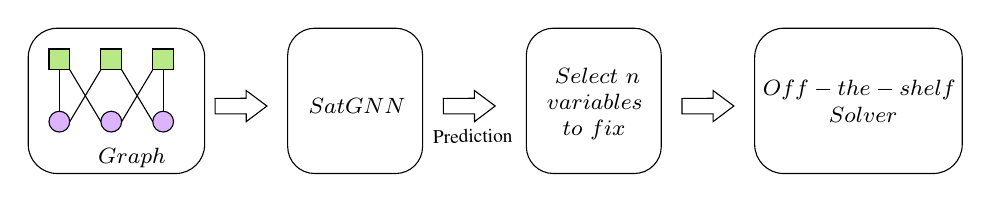
\begin{tikzpicture}[x=0.75pt,y=0.75pt,yscale=-1,xscale=1]
%uncomment if require: \path (0,451); %set diagram left start at 0, and has height of 451

%Shape: Rectangle [id:dp3587479777011455] 
\draw  [fill={rgb, 255:red, 184; green, 233; blue, 134 }  ,fill opacity=1 ] (75,295) -- (85,295) -- (85,305) -- (75,305) -- cycle ;
%Shape: Circle [id:dp623010589573948] 
\draw  [fill={rgb, 255:red, 144; green, 19; blue, 254 }  ,fill opacity=0.32 ] (100,330) .. controls (100,327.24) and (102.24,325) .. (105,325) .. controls (107.76,325) and (110,327.24) .. (110,330) .. controls (110,332.76) and (107.76,335) .. (105,335) .. controls (102.24,335) and (100,332.76) .. (100,330) -- cycle ;
%Shape: Circle [id:dp6210319224354044] 
\draw  [fill={rgb, 255:red, 144; green, 19; blue, 254 }  ,fill opacity=0.32 ] (125,330) .. controls (125,327.24) and (127.24,325) .. (130,325) .. controls (132.76,325) and (135,327.24) .. (135,330) .. controls (135,332.76) and (132.76,335) .. (130,335) .. controls (127.24,335) and (125,332.76) .. (125,330) -- cycle ;
%Shape: Circle [id:dp9356574928412065] 
\draw  [fill={rgb, 255:red, 144; green, 19; blue, 254 }  ,fill opacity=0.32 ] (75,330) .. controls (75,327.24) and (77.24,325) .. (80,325) .. controls (82.76,325) and (85,327.24) .. (85,330) .. controls (85,332.76) and (82.76,335) .. (80,335) .. controls (77.24,335) and (75,332.76) .. (75,330) -- cycle ;
%Shape: Rectangle [id:dp3734262207947956] 
\draw  [fill={rgb, 255:red, 184; green, 233; blue, 134 }  ,fill opacity=1 ] (100,295) -- (110,295) -- (110,305) -- (100,305) -- cycle ;
%Shape: Rectangle [id:dp01885589435556012] 
\draw  [fill={rgb, 255:red, 184; green, 233; blue, 134 }  ,fill opacity=1 ] (125,295) -- (135,295) -- (135,305) -- (125,305) -- cycle ;
%Straight Lines [id:da4907255353964277] 
\draw    (85,305) -- (100,330) ;
%Straight Lines [id:da9596012294566421] 
\draw    (130,305) -- (130,325) ;
%Straight Lines [id:da4248647563144248] 
\draw    (110,305) -- (125,330) ;
%Straight Lines [id:da6077808155610602] 
\draw    (110,330) -- (125,305) ;
%Straight Lines [id:da7849471865454107] 
\draw    (100,305) -- (85,330) ;
%Straight Lines [id:da019130866741998265] 
\draw    (80,305) -- (80,325) ;
%Down Arrow [id:dp06778528901825087] 
\draw   (170.04,330) -- (170.02,326.25) -- (155.03,326.29) -- (155.01,318.79) -- (170,318.75) -- (169.99,315) -- (180.01,322.47) -- cycle ;
%Rounded Rect [id:dp6272397850061886] 
\draw   (65,299) .. controls (65,291.27) and (71.27,285) .. (79,285) -- (136,285) .. controls (143.73,285) and (150,291.27) .. (150,299) -- (150,341) .. controls (150,348.73) and (143.73,355) .. (136,355) -- (79,355) .. controls (71.27,355) and (65,348.73) .. (65,341) -- cycle ;
%Rounded Rect [id:dp6283367026252633] 
\draw   (190,298) .. controls (190,290.82) and (195.82,285) .. (203,285) -- (242,285) .. controls (249.18,285) and (255,290.82) .. (255,298) -- (255,342) .. controls (255,349.18) and (249.18,355) .. (242,355) -- (203,355) .. controls (195.82,355) and (190,349.18) .. (190,342) -- cycle ;
%Rounded Rect [id:dp5504011516450884] 
\draw   (305,298) .. controls (305,290.82) and (310.82,285) .. (318,285) -- (357,285) .. controls (364.18,285) and (370,290.82) .. (370,298) -- (370,342) .. controls (370,349.18) and (364.18,355) .. (357,355) -- (318,355) .. controls (310.82,355) and (305,349.18) .. (305,342) -- cycle ;
%Rounded Rect [id:dp38041408857667824] 
\draw   (415,299) .. controls (415,291.27) and (421.27,285) .. (429,285) -- (501,285) .. controls (508.73,285) and (515,291.27) .. (515,299) -- (515,341) .. controls (515,348.73) and (508.73,355) .. (501,355) -- (429,355) .. controls (421.27,355) and (415,348.73) .. (415,341) -- cycle ;
%Down Arrow [id:dp2151743401001469] 
\draw   (280.01,330) -- (279.99,326.25) -- (265,326.29) -- (264.98,318.79) -- (279.97,318.75) -- (279.96,315) -- (289.98,322.47) -- cycle ;
%Down Arrow [id:dp19599668218528143] 
\draw   (394.99,330) -- (394.98,326.25) -- (379.99,326.29) -- (379.97,318.79) -- (394.96,318.75) -- (394.95,315) -- (404.96,322.47) -- cycle ;

% Text Node
\draw (258.63,332.91) node [anchor=north west][inner sep=0.75pt]  [rotate=-358.87] [align=left] {{\fontfamily{ptm}\selectfont {\scriptsize Prediction}}};
% Text Node
\draw (195,317.4) node [anchor=north west][inner sep=0.75pt]  [font=\footnotesize]  {$~SatGNN$};
% Text Node
\draw (71,341.4) node [anchor=north west][inner sep=0.75pt]  [font=\footnotesize]  {~~~~~~~$Graph$};
% Text Node
\draw (307,301.4) node [anchor=north west][inner sep=0.75pt]  [font=\footnotesize]  {$ \begin{array}{l}
\ Select\ n\ \\
variables\ \\
\ \ to\ fix
\end{array}$};
% Text Node
\draw (411,307.4) node [anchor=north west][inner sep=0.75pt]  [font=\footnotesize]  {$ \begin{array}{c}
Off-the-shelf\ \\
Solver
\end{array}$};


\end{tikzpicture}

}
\caption{Early fixing with SatGNN.}
\label{fig:ef-satgnn}
\end{figure}

Therefore, given a set $\hat{X}$ of random candidate solutions for a given problem instance, we compute \[
\hat{x}^* = \frac{1}{|\hat{X}|}\sum_{\hat{x}\in \hat{X}} \hat{x}\odot \hat{y}(\hat{x}) + (1-\hat{x}) \odot (1 - \hat{y}(\hat{x}))
,\] where $\odot$ is the element-wise product and $\hat{y}(\hat{x})$ is the predicted optimality of candidate solution $\hat{x}\in\hat{X}$ generated using the model from the previous experiment.
In the results reported 

Furthermore, we can say that the closer a given predicted optimal variable $\hat{x}^*_i$ is to 1 (resp. 0), the more certain the model is that that variable should be fixed at 1 (resp. 0).
Therefore, we use the model's certainty to select the variables to be fixed; that is, if we want to fix 50 binary variables, we will choose the 50 variables that the model is most certain of.
We evaluate the accuracy of the SatGNN for early fixing as a function of the number of fixed variables on the two instances of the test set.
These results can be seen in figure \ref{fig:ef-acc}.
As expected, the accuracy decreases as we include variables for which the model is less certain, to the limit of 82.5\% and 87.9\% accuracy on the two instances, which is the accuracy of the predicted optimal solution over the 1745 variables.
A summary of the model's performance when fixing all variables can be seen in Table \ref{tab:exp23-test-performance}.

\begin{figure}[!htb]
    \centering
    \includegraphics[width=0.4\textwidth]{figures/acc_97_9_6.png}
    \includegraphics[width=0.4\textwidth]{figures/acc_97_9_9.png}
    \caption{Early fixing accuracy for the two instances of the ONTS problem in the test set.}
    \label{fig:ef-acc}
\end{figure}

In face of these results, we evaluate how early fixing using SatGNN impacts the optimization performance both in terms of runtime and maximum objective value.
Specifically, we solve the two instances of the ONTS problem on the test set using Gurobi under an increasing number of fixed variables.
The results can be seen in figure \ref{fig:ef-impact}.

\begin{figure}[!htb]
    \centering
    \includegraphics[width=0.4\textwidth]{figures/runtime_obj_97_9_6.png}
    \includegraphics[width=0.4\textwidth]{figures/runtime_obj_97_9_9.png}
    \caption{Optimization results of the two ONTS instances with SatGNN-based early fixing. The objective is plotted with respect to the maximum of the original problem (without any fixed variables). Accuracy is measured with respect to the optimal value of the fixed variables.}
    \label{fig:ef-impact}
\end{figure}

As expected, correctly fixing the variables positively impacts the optimization, while wrongly fixing variables may decrease the runtime but often impacts the objective negatively.
However, we see that, at the limit, a substantial runtime reduction is achieved (90\% and 28\%, for instances 6 and 9, resp.) with a negligible objective cost (1.3\% and 0.3\%, resp.).
Beyond that, fixing more than 500 variables for instance 6 and more than 200 for instance 9 deemed the problems infeasible within a 5 minutes budget.

Given that the SatGNN model could generalize the optimality classification for larger instances of the problem, we also evaluate the impact of early fixing based on our model for the same two larger instances used in the previous experiment.
The performance on the larger instances can be seen in Figure \ref{fig:exp3-larger-instances} and in Table \ref{tab:exp23-test-performance}.
Even though these instances' sizes were not seen during training (not even during validation), the model was still able to handle them and provide sensible early fixing candidates.
The performance drop is significant in terms of accuracy and optimization performance.
In most configurations, however, the model was still able to reduce the runtime with little to no objective value reduction.

\begin{figure}[!htb]
    \centering
    \includegraphics[height=0.3\textwidth]{figures/acc_97_11.png}
    \includegraphics[height=0.3\textwidth]{figures/runtime_obj_97_11.png}
    \includegraphics[height=0.3\textwidth]{figures/acc_120_9.png}
    \includegraphics[height=0.3\textwidth]{figures/runtime_obj_120_9.png}
    \caption{Performance of SatGNN on early fixing instances larger than those seen during training and validation. Instance 97\_11 has 11 jobs, 2 more than the instances previously seen. Instance 120\_9 has the same amount of jobs but schedules for 120-time steps, 23 more than in the instances previously seen.}
    \label{fig:exp3-larger-instances}
\end{figure}

%\subsection{Discussion}

%\section{Conclusions}

\noindent
% We introduce an attack on aggregated gradients that leaks thousands of images within a single training iteration. The promise of secure aggregation is only that an attacker cannot gain access to individual client updates. We show that a malicious server can easily break all types of privacy that aggregation wants to achieve, regardless of the size and number of clients in aggregation.

\begin{comment}
1. We break privacy of secure aggregation in FL setting through server sending customized model updates. 
2. We use leakage through a linear layer, i.e., through the FC layer.
3. Our key design idea is that we send customized convolutional kernels to each client, an identity mapping set, that causes the data to be pushed unchanged through the initial layers. 
4. We are the first to do this at scale. Scale argument.
5. We show empirically that our leakage rate is between 60-70\% with CIFAR-100, Tiny ImageNet, and  MNIST with 100 clients, while that of the state-of-the-art is less than 1\% when the same number of non-zero parameters is used. 
6. We can operate in non-iid setting, which is an important subclass of FL. For this, we learn the client-specific parameters through an initial few updates, often through just a single training round. 
\end{comment}
\noindent
In this paper, we have demonstrated how to break the privacy of secure aggregation in federated learning through a malicious server that sends customized modified models to each client. The attack works by inserting a client-specific convolutional layer followed by two fully connected layers in front of the original application model. Our key design idea is to send customized convolutional kernels to each client, an identity mapping set, that separates the weight gradients of data points between clients despite the use of secure aggregation. The server then uses these weight gradients to reconstruct the original data points. We are the first to achieve a privacy attack in FL that scales well, with the size of the batch and the number of clients. For us to handle an increasing batch size, the fully connected layer size increases linearly and so the number of parameters increases linearly. For us to handle an increasing number of clients, the size of the convolutional layer increases linearly and so the total number of parameters grows linearly, while the number of non-zero parameters stays constant. We show empirically that our leakage rate is between 70-80\% with CIFAR-100, Tiny ImageNet, and  MNIST with 100 clients, while that of the state-of-the-art is less than 1\% when the same number of non-zero parameters is used. 
We can operate in non-IID setting, which is an important subclass of FL. For this, we learn the client-specific parameters through an initial few updates, often through just a single training round. 


\begin{comment}
    
\section*{Acknowledgements}

We thank the Center for Information Technology of the University of Groningen for their support and for providing access to the Peregrine high performance computing cluster.
\end{comment}
%%%%%%%%% REFERENCES
{\small
\bibliographystyle{ieee_fullname}
\bibliography{egbib}
}

\newpage
\appendix

\section{Appendix for Proofs}

\paragraph{Proof of Theorem \ref{thm:main}.}

\begin{proof}
\label{proof:main}
Our proof has two steps. In Step 1, we will show that SimCLR is equivalent to minimizing the cross entropy loss defined in Eqn.~(\ref{eqn:cross-entropy}). 
In Step 2, we will show  that minimizing the cross-entropy loss 
is equivalent to spectral clustering on $\bfpi$. 
Combining the two steps together, we have proved our theorem. 

\textbf{Step 1: } SimCLR is equivalent to minimizing the cross entropy loss.

The cross-entropy loss takes expectation over 
$\bfW_\bfX\sim \mathbb{P}(\cdot ; \bfpi)$, 
which means $\bfW_\bfX$ has exactly one non-zero entry in each row $i$. By Lemma~\ref{lem:multinomial}, we know every row $i$ of $\bfW_\bfX$ is independent of other rows. Moreover, 
$\bfW_{\bfX,i}\sim \mathcal{M}(1, \bfpi_i/\sum_j \bfpi_{i,j})=\mathcal{M}(1, \bfpi_i)$, because $\bfpi_i$ itself is a probability distribution.
Similarly, we know $\bfW_\bfZ$ also has the row-independent property by sampling over $\mathbb{P}(\cdot;\bfK_\bfZ)$.
Therefore, by Lemma~\ref{lem:cross_split}, we know Eqn.~(\ref{eqn:cross-entropy}) is equivalent to:
\[
 -\sum_{i=1}^n \mathbb{E}_{\bfW_{\bfX,i}}[\log \mathbb{P}(\bfW_{\bfZ,i}=\bfW_{\bfX,i};\bfK_\bfZ)],
\]

This expression takes expectation over $\bfW_{\bfX,i}$ for the given row $i$. Notice that 
$\bfW_{\bfX,i}$ has exactly one non-zero entry, which equals $1$ (same for $\bfW_{\bfZ,i}$). 
As a result
we expand the above expression to be:
\begin{equation}
 -\sum_{i=1}^n \sum_{j\neq i} \Pr(\bfW_{\bfX,i,j}=1)\log \Pr(\bfW_{\bfZ,i,j}=1).
\label{eqn:detailed-expansion}    
\end{equation}


By Lemma~\ref{lem:multinomial}, $\Pr(\bfW_{\bfZ,i,j}=1)=\bfK_{\bfZ,i,j}/\|\bfK_{\bfZ,i}\|_1$ for $j\neq i$. Recall that $\bfK_\bfZ=(k(\bfZ_i-\bfZ_j))_{(i,j)\in[n]^2}$, which means 
$\bfK_{\bfZ,i,j}/\|\bfK_{\bfZ,i}\|_1=\frac{\exp(-\|\bfZ_i-\bfZ_j\|^2/{2\tau})}{\sum_{k\neq i}
\exp(-\|\bfZ_i-\bfZ_k\|^2/{2\tau})
}$ for $j\neq i$, when $k$ is the Gaussian kernel with variance $\tau$. 

Notice that $\bfZ_i=f(\bfX_i)$, so we know
\begin{equation}
-\log \Pr(\bfW_{\bfZ,i,j}=1)=
-\log \frac{\exp(-\|f(\bfX_i)-f(\bfX_j)\|^2/{2\tau})}{\sum_{k\neq i}
\exp(-\|f(\bfX_i)-f(\bfX_k)\|^2/{2\tau}),
}
\label{eqn:infonce-equivalence}    
\end{equation}


The right hand side is exactly the InfoNCE loss defined in Eqn.~(\ref{eqn:infonce}).
Inserting Eqn.~(\ref{eqn:infonce-equivalence}) into Eqn.~(\ref{eqn:detailed-expansion}), we get the SimCLR algorithm, which first samples augmentation pairs $(i,j)$ with $\Pr(\bfW_{\bfX,i,j}=1)$ for each row $i$, and then optimize the InfoNCE loss. 

\textbf{Step 2: } minimizing the cross entropy loss 
is equivalent to spectral clustering on $\bfpi$.


By Lemma~\ref{lem:convert_to_spectral}, we may further convert the loss to 
\begin{equation}
\label{eqn:main-theorem-repul-attr}
\min_{\bfZ}
-\sum_{(i,j)\in [n]^2} \mathbf{P}_{i,j}
\log k (\bfZ_i-\bfZ_j)+\log \mathbf{R}(\bfZ).
\end{equation}
Since $k$ is the Gaussian kernel, this reduces to \[
\min_\bfZ \mathrm{tr}(\bfZ^\top \mathbf{L}(\bfpi) \bfZ)
+\log \mathbf{R}(\bfZ),
\]

where we use the fact that $\mathbb{E}_{\bfW_\bfX\sim \mathbb{P}(\cdot; \bfpi)}[\mathbf{L}(\bfW_\bfX)]
=\mathbf{L}(\bfpi)
$, because the Laplacian operator is linear and $
\mathbb{E}_{\bfW_\bfX\sim \mathbb{P}(\cdot; \bfpi)}(\bfW_\bfX)=\bfpi
$.
\end{proof}

\paragraph{Proof of Theorem \ref{thm:clip}.}
\begin{proof}
Since $\bfW_\bfX\sim \mathbb{P}(\cdot;\bfpi_{\mathbf{A}, \mathbf{B}})$, we know 
$\bfW_\bfX$ has exactly one non-zero entry in each row, denoting the pair that got sampled. 
A notable difference compared to the previous proof is we now have $n_\mathcal{A}+n_\mathcal{B}$ objects in our graph. CLIP deals with this by taking a mini-batch of size $2N$, 
such that $n_\mathcal{A}=n_\mathcal{B}=N$, and adding the $2N$ InfoNCE losses together. We label the objects in $\mathcal{A}$ as $[n_\mathcal{A}]$, and the objects in $\mathcal{B}$ as $\{n_\mathcal{A}+1, \cdots, n_\mathcal{A}+n_\mathcal{B}\}$. 

Notice that $\bfpi_{\mathbf{A}, \mathbf{B}}$ is a bipartite graph, so the edges of objects in $\mathcal{A}$ will only connect to object in $\mathcal{B}$ and vice versa. We can define the similarity matrix in $\cZ$ as $\bfK_\bfZ$, 
where $\bfK_\bfZ(i, j+n_\mathcal{A})=\bfK_\bfZ(j+n_\mathcal{A},i)= k(\bfZ_i-\bfZ_j)$ for $i\in [n_\mathcal{A}], j\in [n_\mathcal{B}]$, and otherwise we set $\bfK_\bfZ(i,j)=0$. 
The rest is same as the previous proof. 
\end{proof}

\paragraph{Proof of Theorem \ref{thm:exponential}.}

\begin{proof}
\label{proof:exponential}
Since the objective function consists of a linear term combined with an entropy regularization, which is a strongly concave function, the maximization problem is a convex optimization problem. Owing to the implicit constraints provided by the entropy function, the problem is equivalent to having only the equality constraint. We then introduce the Lagrangian multiplier $\lambda$ and obtain the following relaxed problem:

$$
\widetilde{E}(\boldsymbol{\alpha})=\psi_{1}-\sum_{i=1}^n \alpha_{i} \psi_{i}+\tau \sum_{i=1}^n \alpha_{i}\log \alpha_{i}+\lambda\left(\boldsymbol{\alpha}^{\top} \mathbf{1}_n-1\right).
$$

As the relaxed problem is unconstrained, taking the derivative with respect to $\alpha_{i}$ yields

$$
\frac{\partial \widetilde{E}(\boldsymbol{\alpha})}{\partial \alpha_{i}}=-\psi_{i}+\tau\left(\log \alpha_{i}+\alpha_{i} \frac{1}{\alpha_{i}}\right)+\lambda=0.
$$

Solving the above equation implies that $\alpha_{i}$ takes the form
$
\alpha_{i}=\exp \left(\frac{1}{\tau} \psi_{i}\right) \exp \left(\frac{-\lambda}{\tau}-1\right).
$ Since $\alpha_{i}$ lies on the probability simplex, the optimal $\alpha_{i}$ is explicitly given by
$
\alpha^{*}_{i}=\frac{\exp \left(\frac{1}{\tau} \psi_{i}\right)}{\sum_{i^{\prime}=1}^n \exp \left(\frac{1}{\tau} \psi_{i^{\prime}}\right)} .
$ Substituting the optimal point into the objective function, we obtain
$$
\begin{aligned}
E\left(\boldsymbol{\alpha}^*\right)  &=\psi_1-\sum_{i=1}^n \frac{\exp \left(\frac{1}{\tau} \psi_{i}\right)}{\sum_{i^{\prime}=1}^n \exp \left(\frac{1}{\tau} \psi_{i^{\prime}}\right)} \psi_{i}+\tau \sum_{i=1}^n \frac{\exp \left(\frac{1}{\tau} \psi_{i}\right)}{\sum_{i^{\prime}=1}^n \exp \left(\frac{1}{\tau} \psi_{i^{\prime}}\right)}\log \frac{\exp \left(\frac{1}{\tau} \psi_{i}\right)}{\sum_{i^{\prime}=1}^n \exp \left(\frac{1}{\tau} \psi_{i^{\prime}}\right)} \\
& =\psi_1 - \tau \log \left(\sum_{i=1}^n \exp \left(\frac{1}{\tau} \psi_{i}\right)\right).
\end{aligned}
$$
Thus, the Lagrangian dual function is given by
\begin{equation*}
-E\left(\boldsymbol{\alpha}^*\right)= -\tau \log \frac{\exp \left(\frac{1}{\tau} \psi_{1}\right)}{\sum_{i=1}^n \exp \left(\frac{1}{\tau} \psi_{i}\right)}.\qedhere
\end{equation*}
\end{proof}



\section{More on Experiments} \label{section: experiment_details}

\paragraph{CIFAR-10 and CIFAR-100} CIFAR-10 ~\citep{krizhevsky2009learning} and CIFAR-100 ~\citep{krizhevsky2009learning} are well-known classic image classification datasets. Both CIFAR-10 and CIFAR-100 contain a total of 60k $32 \times 32$ labeled images of different classes, with 50k for training and 10k for testing. CIFAR-10 is similar to CIFAR-100, except there are 10 different classes in CIFAR-10 and 100 classes in CIFAR-100.

\paragraph{TinyImageNet} TinyImageNet ~\citep{le2015tiny} is a subset of ImageNet ~\citep{deng2009imagenet}. There are 200 different object classes in TinyImageNet, with 500 training images, 50 validation images, and 50 test images for each class. All the images in TinyImageNet are colored and labeled with a size of $64 \times 64$.

\textbf{Pseudo-code.} Algorithm \ref{alg:Training Procedure} presents the pseudo-code for our empirical training procedure.

\begin{algorithm}[!htbp]
\caption{Training Procedure}
\label{alg:Training Procedure}
\begin{algorithmic}[1]
\REQUIRE trainable encoder network $f$, batch size $N$, augmentation strategy \textit{aug}, loss function $L$ with hyperparameters \textit{args}
\FOR {sampled minibatch ${x_i}_{i=1}^N$}
\FORALL{$i \in { 1, ..., N }$}
\STATE draw two augmentations $t_i = \textit{aug}\left(x_i\right) $, $t_i' = \textit{aug}\left(x_i\right) $
\STATE $z_i = f\left(t_i\right)$, $z_i' = f\left(t_i'\right)$
\ENDFOR
\STATE compute loss $\mathcal{L} = L(N, z, z', \textit{args})$
\STATE update encoder network $f$ to minimize $\mathcal{L}$
\ENDFOR
\STATE \textbf{Return} encoder network $f$
\end{algorithmic}
\end{algorithm}

We also provide the pseudo-code for our core loss function used in the training procedure in Algorithm \ref{alg:Core loss}. The pseudo-code is almost identical to SimCLR's loss function, with the exception of an extra parameter $\gamma$.

\begin{algorithm}[!htbp]
\caption{Core loss function $\mathcal{C}$}
\label{alg:Core loss}
\begin{algorithmic}[1]
\REQUIRE batch size $N$, two encoded minibatches $z_1, z_2$, $\gamma$, temperature $\tau$
\STATE $z = \textit{concat}\left(z_1, z_2\right)$
\FOR {$i \in {1, ..., 2N }, j \in {1, ..., 2N}$ }
\STATE $s_{i,j} = \Vert z_i - z_j \Vert_2^{\gamma}$
\ENDFOR
\STATE \textbf{define} $l(i, j)$ \textbf{as} $l(i, j) = - \log \frac{exp\left(s_{i,j}/\tau \right)}{\sum_{k=1}^{2N} \mathbf{1}{[k \ne i]} exp\left(s{i, j} / \tau \right)} $
\STATE \textbf{Return} $\frac{1}{2N} \sum_{k=1}^N\left[l(i, i+N) + l(i+N, i)\right]$
\end{algorithmic}
\end{algorithm}

Utilizing the core loss function $\mathcal{C}$, we can define all kernel loss functions used in our experiments in Table \ref{table: loss definition}. For all $z_i \in z$ with even dimensions $n$, we define $z_{L_i} = z_i\left[0:n/2\right]$ and $z_{R_i} = z_i\left[n/2:n\right]$.

\begin{table}[ht]
\centering
\begin{tabular}{{@{}l|l@{}}}
Kernel  &  Loss function \\ \midrule
Laplacian & $\mathcal{C}\left(N, z, z', \gamma=1, \tau\right)$\\ \midrule
Sum       & $\lambda * \mathcal{C}\left(N, z, z', \gamma=1, \tau_1\right) + (1-\lambda) * \mathcal{C}\left(N, z, z', \gamma=2, \tau_2\right)$  \\ \midrule
Concatenation Sum&$\lambda * \mathcal{C}\left(N, z_L, z'_L, \gamma=1, \tau_1\right) + (1-\lambda) * \mathcal{C}\left(N, z_R, z'_R, \gamma=2, \tau_2\right)$\\ \midrule
$\gamma = 0.5$ & $\mathcal{C}\left(N, z, z', \gamma=0.5, \tau\right)$          \\ 

\end{tabular}

\caption{Definition of kernel loss functions in our experiments}
\label {table: loss definition}
\end{table}

\textbf{Baselines.} We reproduce the SimCLR algorithm using PyTorch Lightning~\citep{PytorchLightning}.

\textbf{Encoder details.}
The encoder $f$ consists of a backbone network and a projection network. We employ ResNet50~\citep{ResNet} as the backbone and a 2-layer MLP (connected by a batch normalization~\citep{ioffe2015batch} layer and a ReLU \cite{nair2010rectified} layer) with hidden dimensions 2048 and output dimensions 128 (or 256 in the concatenation kernel case).

\textbf{Encoder hyperparameter tuning.}
For each encoder training case, we randomly sample 500 hyperparameter groups (sample details are shown in Table \ref{table: Hyperparameter sample}) and train these samples simultaneously using Ray Tune ~\citep{RayTune}, with the ASHA scheduler~\citep{li2018massively}. Ultimately, the hyperparameter group that maximizes the online validation accuracy (integrated in PyTorch Lightning) within 5000 validation steps is chosen for the given encoder training case.

\begin{table}[ht]
\centering

\begin{tabular}{@{}l|l|l@{}}
\midrule
Hyperparameter  & Sample Range & Sample Strategy \\ \midrule
start learning rate & $\left[10^{-2}, 10\right]$ & log uniform \\ \midrule
$\lambda$       & $\left[0, 1\right]$ & uniform \\ \midrule
$\tau$, $\tau_1$, $\tau_2$ & $\left[0, 1\right]$ & log uniform \\ \midrule
\end{tabular}

\caption{Hyperparameters sample strategy}
\label {table: Hyperparameter sample}
\end{table}

\textbf{Encoder training.} 
We train each encoder using the LARS optimizer~\citep{LARSOptimizer}, LambdaLR Scheduler in PyTorch, momentum 0.9, weight decay $10^{-6}$, batch size 256, and the aforementioned hyperparameters for 400 epochs on a single A-100 GPU.

\textbf{Image transformation.} The image transformation strategy, including augmentation, is identical to the default transformation strategy provided by PyTorch Lightning.

\textbf{Linear evaluation.}
The linear head is trained using the SGD optimizer with a cosine learning rate scheduler, batch size 64, and weight decay $10^{-6}$ for 100 epochs. The learning rate starts at $0.3$ and ends at $0$.

\textbf{Moco Experiments.} We also tested our method based on MoCo~\citep{he2019moco}. The results are summarized in Table \ref{tab:results-moco}. Here we choose ResNet18~\citep{ResNet} as the backbone and set a temperature of $0.1$ as default. For our simple sum kernel, we set $\lambda=0.8$. The results show that our method outperforms the original MoCo method.

\begin{table}[thb]
\centering
\caption{MoCo Experiment Results on CIFAR-10 and CIFAR-100.}
\label{tab:results-moco}
\resizebox{\textwidth}{!}{%
\begin{tabular}{@{}c|ccc|ccc@{}}
\toprule
\multirow{3}{*}{Method} & \multicolumn{3}{c|}{CIFAR-10} & \multicolumn{3}{c}{CIFAR-100} \\ \cmidrule(lr){2-4} \cmidrule(lr){5-7} 
                        & 200 epochs & 400 epochs    & 1000 epochs   & 200 epochs & 400 epochs & 1000 epochs         \\ \midrule
MoCo (repro.)         & $76.41 \pm 0.12$    & $80.01 \pm 0.15$          & $84.45 \pm 0.08$    & $\mathbf{47.02 \pm 0.11}$ & $52.50 \pm 0.07$ & $57.62 \pm 0.15$            \\
\midrule
Laplacian Kernel        & ${78.09 \pm 0.10}$    & $\mathbf{83.85 \pm 0.09}$          & $\mathbf{88.34 \pm 0.16}$    & $46.12 \pm 0.22$   & $53.44 \pm 0.17$ & $59.10 \pm 0.14$        \\
Simple Sum Kernel & $\mathbf{78.12 \pm 0.15}$   & $83.23 \pm 0.18$ & $87.50 \pm 0.20$ & $46.65 \pm 0.06$ & $\mathbf{53.62 \pm 0.19}$ & $\mathbf{59.83 \pm 0.12}$\\
\bottomrule
\end{tabular}
}
\end{table}



\section{More Experiments on Synthetic Data}


Consider a scenario with $n$ clusters, each containing $k$ vertices. Let the probability of vertices $u$ and $v$ from the same cluster belonging to $\bfpi$ be $p$. Conversely, for vertices $u$ and $v$ from different clusters, let the probability of belonging to $\pi$ be $q$. We generate the graph $\bfpi$ randomly, based on $p$ and $q$. We experiment with values of $k=100$ and $n=6$ for ease of visualization, embedding all points in a two-dimensional space. Each vertex's initial position originates from a normal distribution. In each iteration, we sample a subgraph of $\bfpi$ uniformly, ensuring each vertex has an out-degree of $1$. We then optimize the corresponding vectors using InfoNCE loss with an SGD optimizer and iterate until convergence. Our experimental setup consists of an SGD learning rate of $1$, an InfoNCE loss temperature of $0.5$, and a batch size of $50$. We evaluate two scenarios with different $p$ and $q$ values: $p=1$, $q=0$, and $p=0.75$, $q=0.2$. The results of these experiments are visualized in Figure \ref{fig:vis-spectral-cluster}. The obtained embeddings exhibit the hallmark pattern of spectral clustering of graph $\bfpi$.

\begin{figure}[!tb]
\centering
\subfigure{
\includegraphics[width=1\textwidth]{Figures/cluster_pi.png}
\label{fig:vis-cluster}
}
\subfigure{
\includegraphics[width=1\textwidth]{Figures/noised_cluster_pi.png}
\label{fig:vis-noised-cluster}
}
\caption{Visualizations of the optimization process using InfoNCE Loss on the vectors corresponding to $\bfpi$. Points of identical color belong to the same cluster within $\bfpi$. To showcase the internal structure of $\bfpi$, we randomly select 10 vertices from each cluster to display the edge distribution of $\bfpi$.}
\label{fig:vis-spectral-cluster}
\end{figure}


%\bibliographystyle{spmpsci}
%\bibliography{egbib}


\end{document}